\documentclass[13pt,oneside]{book}
\usepackage[utf8]{inputenc}
\usepackage{url}
\usepackage{graphicx}
\usepackage{listings}
\usepackage{geometry}
\geometry{a4paper, left=20mm, right=20mm, top=20mm, bottom=20mm}
\usepackage[toc,page]{appendix}
\usepackage{graphicx}
\usepackage{natbib}
\usepackage{lipsum}
\usepackage{caption}

\begin{document}

\captionsetup[figure]{margin=1.5cm,font=small,labelfont={bf},name={Figure},labelsep=colon,textfont={it}}
\captionsetup[table]{margin=1.5cm,font=small,labelfont={bf},name={Table},labelsep=colon,textfont={it}}
\setlipsumdefault{1}

\begin{titlepage}
\begin{center}
{\LARGE College Of Engineering Trivandrum}\\[3cm]
\linespread{1.2}\huge {\bfseries System Software Lab}\\[3cm]
\linespread{1}

\includegraphics[width=5cm]{img/emblem.jpeg}\\[3cm]
{\Large Gokul K\\ S5  CSE \\ Roll No:21\\ TVE18CS021 }\\[1cm]


\textit{ }\\[2cm]
Department of Computer Science\\[0.2cm]
\today
\end{center}

\end{titlepage}

\newpage
\large
\noindent{\bfseries{\huge Contents}\hfill Page No.\vspace \bigskipamount \par }
\contentsline {chapter}{\numberline {1}Cpu Scheduling Algorithms}{3}
\contentsline {section}{\numberline {1.1}Aim}{3}
\contentsline {section}{\numberline {1.2}Algorithm}{3}
\contentsline {section}{\numberline {1.3}Source Code}{5}
\contentsline {section}{\numberline {1.4}Result}{10}
\contentsline {chapter}{\numberline {2}Disk Scheduling Algorithms}{13}
\contentsline {section}{\numberline {2.1}Aim}{13}
\contentsline {section}{\numberline {2.1}Algorithm}{13}
\contentsline {section}{\numberline {2.3}Source Code}{14}
\contentsline {section}{\numberline {2.4}Result}{16}
\contentsline {chapter}{\numberline {3}Page Replacement Algorithms}{17}
\contentsline {section}{\numberline {3.1}Aim}{17}
\contentsline {section}{\numberline {3.2}Algorithm}{17}
\contentsline {section}{\numberline {3.3}Source Code}{18}
\contentsline {section}{\numberline {3.4}Result}{21}
\contentsline {chapter}{\numberline {4}Banker’s Algorithm}{23}
\contentsline {section}{\numberline {4.1}Aim}{23}
\contentsline {section}{\numberline {4.2}Algorithm}{23}
\contentsline {section}{\numberline {4.3}Source Code}{23}
\contentsline {section}{\numberline {4.4}Result}{26}
\contentsline {chapter}{\numberline {5}Producer Consumer Problem}{27}
\contentsline {section}{\numberline {5.1}Aim}{27}
\contentsline {section}{\numberline {5.2}Algorithm}{27}
\contentsline {section}{\numberline {5.3}Source Code}{27}
\contentsline {section}{\numberline {5.4}Result}{29}
\contentsline {chapter}{\numberline {6}Dining Philosophers Problem}{30}
\contentsline {section}{\numberline {6.1}Aim}{30}
\contentsline {section}{\numberline {6.2}Algorithm}{30}
\contentsline {section}{\numberline {6.3}Source Code}{30}
\contentsline {section}{\numberline {6.4}Result}{32}
\contentsline {chapter}{\numberline {7}File Organisation Techniques}{33}
\contentsline {section}{\numberline {7.1}Aim}{33}
\contentsline {section}{\numberline {7.2}Algorithm}{33}
\contentsline {section}{\numberline {7.3}Source Code}{33}
\contentsline {section}{\numberline {7.4}Result}{38}
\contentsline {chapter}{\numberline {8}Pass 1 of a two pass assembler}{40}
\contentsline {section}{\numberline {8.1}Aim}{40}
\contentsline {section}{\numberline {8.2}Algorithm}{40}
\contentsline {section}{\numberline {8.3}Source Code}{41}
\contentsline {section}{\numberline {8.4}Result}{42}
\contentsline {chapter}{\numberline {9}Pass 2 of a two pass assembler}{43}
\contentsline {section}{\numberline {9.1}Aim}{43}
\contentsline {section}{\numberline {9.2}Theory}{43}
\contentsline {section}{\numberline {9.3}Source Code}{44}
\contentsline {section}{\numberline {9.4}Result}{47}
\contentsline {chapter}{\numberline {10}One Pass Assembler}{48}
\contentsline {section}{\numberline {10.1}Aim}{48}
\contentsline {section}{\numberline {10.2}Theory}{48}
\contentsline {section}{\numberline {10.3}Source Code}{48}
\contentsline {section}{\numberline {10.4}Result}{51}
\contentsline {chapter}{\numberline {11}Symbol Table Hashing}{52}
\contentsline {section}{\numberline {11.1}Aim}{52}
\contentsline {section}{\numberline {11.2}Algorithm}{52}
\contentsline {section}{\numberline {11.3}Source Code}{52}
\contentsline {section}{\numberline {11.4}Result}{57}
\contentsline {chapter}{\numberline {12}Implementation of Absolute Loader}{59}
\contentsline {section}{\numberline {12.1}Aim}{59}
\contentsline {section}{\numberline {12.2}Algorithm}{59}
\contentsline {section}{\numberline {12.3}Source Code}{59}
\contentsline {section}{\numberline {12.4}Result}{61}
\contentsline {chapter}{\numberline {13}Implementation of Relocating Loader}{62}
\contentsline {section}{\numberline {13.1}Aim}{62}
\contentsline {section}{\numberline {13.2}Algorithm}{62}
\contentsline {section}{\numberline {13.3}Source Code}{62}
\contentsline {section}{\numberline {13.4}Result}{65}
\contentsline {chapter}{\numberline {14}Implementation of Two Pass Macro Filter}{66}
\contentsline {section}{\numberline {14.1}Aim}{66}
\contentsline {section}{\numberline {14.2}Algorithm}{66}
\contentsline {section}{\numberline {14.3}Source Code}{66}
\contentsline {section}{\numberline {14.4}Result}{69}
\newpage

\begin{frame}{}
    \centering
    \hspace*{-0.5cm}
    $\vcenter{\hbox{
\includegraphics[width=1.5cm]{img/emblem.jpeg}}}$
    $\vcenter{\resizebox{0.95\textwidth}{!}{
        \begin{tabular}{c}
             CS333 - System Software Lab $\cdot$ 2020 $\cdot$   \\
             \hline 
        \end{tabular}
    }}$
\end{frame}
\section*{Cycle 1}
\section*{Expt 1}
\begin{center}
    \Large{CPU Scheduling Algorithms}
\end{center}

\section*{Aim}
\large{
Simulate the following non-preemptive CPU Scheduling
Algorithms to find turnaround time and waiting time.\\
a) FCFS\\
b) SJF\\
c) Round Robin (pre-emptive)\\
d) Priority\\
}

\section*{Algorithm}
    \subsection*{FCFS}
	    \begin{verbatim}
	        1 Start .
            2 Input the processes along with their burst time ( bt ) and
                arrival time ( at ) .
            3 Find the waiting time ( wt ) for all processes .
            4 As process that arrives first need not wait , wt for that process
                will be 0 , wt [0] = 0.
            5 Calculate the wt for all other processes as :
            6 For process i , wt [ i ] = 
                ( bt [0] + bt [1] + .... + bt [i -1]) - at [ i ]
            7 Find turnaround time ( tat ) for all processes .
            8 For process i , tat [ i ] = wt [ i ] + bt [ i ]
            9 Compute average waiting time as ( total_wt / no_of_processes ) .
            10 Compute average turnaround time as ( total_tat / no_of_processes ) .
            11 Stop .
	   \end{verbatim}  
    \subsection*{SJF}
        \begin{verbatim}
            1 Start
            2 Input the processes along with their burst time ( bt ) .
            3 Sort the processes in ascending order of their burst times .
            4 Find the waiting time ( wt ) for all processes .
            5 As the process with smallest bt is scheduled first , it need
                not wait ,
            6 so wt for that process will be 0 , wt [0] = 0.
            7 Calculate the wt for all other processes as :
            8 For process i , wt [ i ] = wt [i -1] + bt [i -1]
            9 Find turnaround time ( tat ) for all processes .
            10 For process i , tat [ i ] = wt [ i ] + bt [ i ]
            11 Compute average waiting time as ( total_wt / no_of_processes ) .
            12 Compute average turnaround time as ( total_tat / no_of_processes ) .
            13 Stop .
        \end{verbatim}  
        
    \subsection*{Round Robin}
        \begin{verbatim}
            1 Start
            2 Input the processes along with their burst time ( bt ) .
            3 Input the time quantum , tq .
            4 Create an array rem_bt [] to keep track of the remaining burst time
                of processes . This array is initially a copy of bt [].
            5 Create another array wt [] to store the waiting times of processes .
            6 Initialize this array as 0.
            7 Initialize time t = 0.
            8 Keep traversing all the processes while all processes are not done
                yet . Do the following for the i th process if it is not done yet
            9 If rem_bt [ i ] > tq
            10 t = t + tq
            11 rem_bt [ i ] = tq
            12 Else
            13 t = t + rem_bt [ i ]
            14 wt [ i ] = t - bt [ i ]
            15 rem_bt [ i ] = 0
            16 // Last cycle for this process
            17 // This process is over
            18 Find turnaround time ( tat ) for all processes .
            19 For process i , tat [ i ] = wt [ i ] + bt [ i ]
            20 Compute average waiting time as ( total_wt / no_of_processes ) .
            21 Compute average turnaround time as ( total_tat / no_of_processes ) .
            22 Stop .
        \end{verbatim}
        
    \subsection*{Priority}
        \begin{verbatim}
            1 Start .
            2 Input the processes along with their burst time ( bt ) and priority .
            3 Sort the processes in ascending order of their priorities .
            4 Find the waiting time ( wt ) for all processes .
            5 As the process with highest priority is scheduled first , it need
                not
            6 wait , so wt for that process will be 0 , wt [0] = 0.
            7 Calculate the wt for all other processes as :
            8 For process i , wt [ i ] = wt [i -1] + bt [i -1]
            9 Find turnaround time ( tat ) for all processes .
            10 For process i , tat [ i ] = wt [ i ] + bt [ i ]
            11 Compute average waiting time as ( total_wt / no_of_processes ) .
            12 Compute average turnaround time as ( total_tat / no_of_processes ) .
            13 Stop .
        \end{verbatim}
\section*{Source Code}
\Large\textbf{process.c}
\small

\begin{lstlisting}[language=C]
#include <stdio.h>
#include <stdlib.h>
#include "process.h"

Process_ptr read_process()
{
	Process_ptr process_ptr = malloc(sizeof(Process));
	scanf(
		"%d %d %d %d", 
		&(process_ptr->p_num),
		&(process_ptr->arrival_time),
		&(process_ptr->execute_time),
		&(process_ptr->priority)
	);
	process_ptr->turnaround_time = process_ptr->waiting_time = 0;
	process_ptr->rem_time = process_ptr->execute_time;
	return process_ptr;
}

Process_list * read_process_list()
{
	/* The list must be sorted by arrival time.
	Hence insertion sort is used */
	size_t length, i;
	short int j;
	Process_ptr key, process_itr;
	Process_ptr *processes;
	Process_list *process_list = malloc(sizeof(Process_list));

	printf("Enter number of processes: ");
	scanf("%d", &(process_list->length));

	process_list->processes = malloc(
	    process_list->length * sizeof(Process_ptr *)
	);
	processes = process_list->processes;

	printf("\nEnter process number, arrival time, execution time and
	priority"
	"\nfor the process. Each value must be seperated by a space\n");
	for(i = 0; i < process_list->length; ++i)
	{
		printf("Process%d: ", i);
		*(processes+i) = read_process();
		key = *(processes+i);
		
		j = i-1;

		while(j >= 0 && 
		    processes[j]->arrival_time > key->arrival_time)
		{
			process_itr = *(processes+j);

			*(processes+j+1) = process_itr;
			--j;
		}
		*(processes+j+1) = key;
	}

	return process_list;
}

void comp_avg_times(Process_list * process_list)
{
	float avg_turnaround_time = 0.0;
	float avg_waiting_time = 0.0;

	for(size_t i = 0; i < process_list->length; i++)
	{
		avg_turnaround_time += 
		    process_list->processes[i]->turnaround_time;
		avg_waiting_time += 
		    process_list->processes[i]->waiting_time;
	}

	avg_turnaround_time /= process_list->length;
	avg_waiting_time /= process_list->length;

	printf(
		"\nAverage waiting time: %.2fu"
		"\nAverage turn-around time: %.2fu\n",
		avg_waiting_time,
		avg_turnaround_time
	);
}

int comp_total_rem_time(Process_list * process_list)
{
	int rem_time = 0;
	for(size_t i = 0; i < process_list->length; i++)
	{
		rem_time += process_list->processes[i]->rem_time;
	}
	return rem_time;
}

    \end{lstlisting}
    
\Large\textbf{schedule.c}
\small
\begin{lstlisting}[language=C]
#include "process.h"
#include <stddef.h>
#include <stdio.h>

void draw_gantt_cell(int p_num, int second, int start_cell, int end_cell) {
  if (start_cell)
    printf("\nGantt Chart (Not-to-scale): ");

  printf("\n----------   t=%du", second);
  printf("\n|P%*d|", 8, p_num);

  if (end_cell)
    printf("\n----------   t=%du\n\n", end_cell);
}

int fcfs(Process_list *process_list) {
  size_t i;
  Process_ptr process_ptr;
  int curr_time = process_list->processes[0]->arrival_time;

  for (i = 0; i < process_list->length; ++i) {
    process_ptr = process_list->processes[i];

    draw_gantt_cell(process_ptr->p_num, curr_time, i == 0,
                    (i == process_list->length - 1)
                        ? curr_time + process_ptr->execute_time
                        : 0);

    process_ptr->waiting_time = curr_time - process_ptr->arrival_time;
    process_ptr->turnaround_time =
        process_ptr->waiting_time + process_ptr->execute_time;
    process_ptr->rem_time = 0;
    curr_time += process_ptr->execute_time;
  }
}

int sjf(Process_list *process_list) {
  size_t i, j;
  Process_ptr process_ptr, process_itr;

  int curr_time = process_list->processes[0]->arrival_time;
  for (i = 0; i < process_list->length; ++i) {
    process_ptr = process_list->processes[i];
    for (j = 0; j < process_list->length; j++) {
      process_itr = process_list->processes[j];
      if (!(process_ptr->rem_time) ||
          process_itr->rem_time && process_itr->arrival_time <= curr_time &&
              process_itr->execute_time < process_ptr->execute_time) {
        process_ptr = process_itr;
      }
    }

    draw_gantt_cell(process_ptr->p_num, curr_time, i == 0,
                    (i == process_list->length - 1)
                        ? curr_time + process_ptr->execute_time
                        : 0);
    process_ptr->waiting_time = curr_time - process_ptr->arrival_time;
    process_ptr->turnaround_time =
        process_ptr->waiting_time + process_ptr->execute_time;
    process_ptr->rem_time = 0;
    curr_time += process_ptr->execute_time;
  }
}

int round_robin(Process_list *process_list, int quantum_time) {
  int total_rem_time = comp_total_rem_time(process_list);
  int instant_work_done, curr_time = 0;

  int last_processed_time[process_list->length];
  Process_ptr process_ptr;
  size_t i;

  // Initialize with all zero
  for (i = 0; i < process_list->length; ++i)
    last_processed_time[i] = 0;

  while (total_rem_time > 0) {
    for (i = 0; i < process_list->length; i++) {
      process_ptr = process_list->processes[i];
      if (!process_ptr->rem_time)
        continue;

      instant_work_done = (process_ptr->rem_time > quantum_time)
                              ? quantum_time
                              : process_ptr->rem_time;
      total_rem_time -= instant_work_done;
      process_ptr->rem_time -= instant_work_done;
      draw_gantt_cell(
          process_ptr->p_num, curr_time, curr_time == 0,
          (total_rem_time == 0 ? curr_time + instant_work_done : 0));
      process_ptr->waiting_time += curr_time - last_processed_time[i];
      process_ptr->turnaround_time +=
          curr_time - last_processed_time[i] + instant_work_done;

      curr_time += instant_work_done;
      last_processed_time[i] = curr_time;
    }
  }
}

int priority(Process_list *process_list) {
  size_t i, j;
  Process_ptr process_ptr, process_itr;

  int curr_time = process_list->processes[0]->arrival_time;
  for (i = 0; i < process_list->length; ++i) {
    process_ptr = process_list->processes[i];  
    for (j = 0; j < process_list->length; j++) {
      process_itr = process_list->processes[j];
      if (!(process_ptr->rem_time) ||
          process_itr->rem_time && process_itr->arrival_time <= curr_time &&
              process_itr->priority < process_ptr->priority) {
        process_ptr = process_itr;
      }
    }

    draw_gantt_cell(process_ptr->p_num, curr_time, i == 0,
                    (i == process_list->length - 1)
                        ? curr_time + process_ptr->execute_time
                        : 0);
    process_ptr->waiting_time = curr_time - process_ptr->arrival_time;
    process_ptr->turnaround_time =
        process_ptr->waiting_time + process_ptr->execute_time;
    process_ptr->rem_time = 0;
    curr_time += process_ptr->execute_time;
  }
}
\end{lstlisting}
\Large\textbf{main.c}
\small
\begin{lstlisting}[language=C]
#include <stdio.h>

#include "process.h"
#include "schedule.h"


int main()
{
	int quantum_time, choice;
	Process_list * process_list = read_process_list();

	printf(
		"Select the scheduling algorithm:"
		"\n\t1) First Come First Serve"
		"\n\t2) Shortest Job First"
		"\n\t3) Round Robin (pre-emptive)"
		"\n\t4) Priority\n"
	);
	scanf("%d", &choice);
	switch (choice)
	{
		case 1:
			fcfs(process_list);
			break;

		case 2:
			sjf(process_list);
			break;
		
		case 3:
			printf("\nEnter quantum time: ");
			scanf("%d", &quantum_time);
			round_robin(process_list, quantum_time);
			break;

		case 4:
			priority(process_list);
			break;

		default:
			break;
	}

	comp_avg_times(process_list);
}

\end{lstlisting}
\section*{Output}
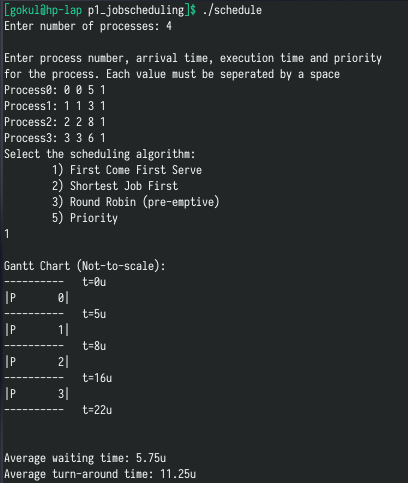
\includegraphics[]{img/p1/ss1.png} \\
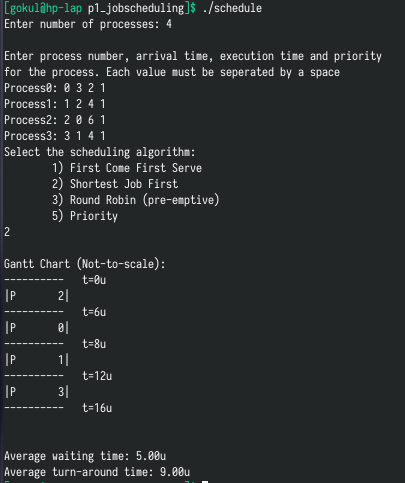
\includegraphics[]{img/p1/ss2.png} \\
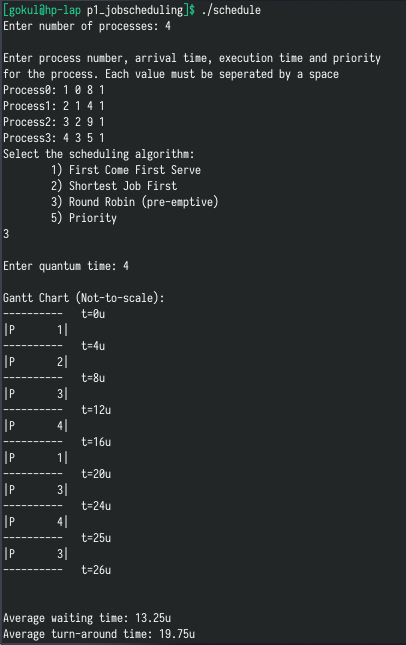
\includegraphics[]{img/p1/ss3.png} \\
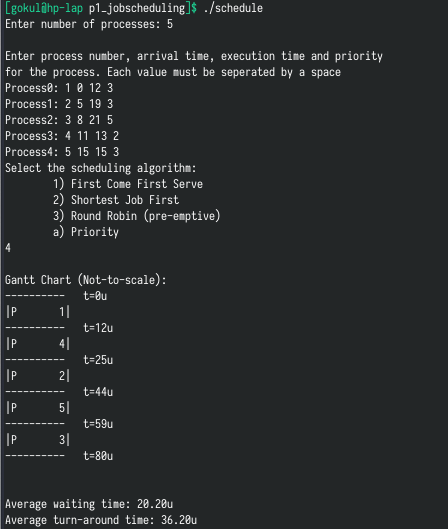
\includegraphics[]{img/p1/ss4.png}

\Large
\section*{Result}
\large
The above algorithms were implemented and its output verified


			\newpage

			\begin{frame}{}
				\centering
				\hspace*{-0.5cm}
				$\vcenter{\hbox{
\includegraphics[width=1.5cm]{img/emblem.jpeg}}}$
				$\vcenter{\resizebox{0.95\textwidth}{!}{
					\begin{tabular}{c}
						 CS333 - System Software Lab $\cdot$ 2020 $\cdot$   \\
						 \hline 
					\end{tabular}
				}}$
			\end{frame}
			\section*{Cycle 1}
\section*{Expt 2}
\begin{center}
    \Large{Disk Scheduling Algorithms}
\end{center}
\section*{Aim}
\large
Simulate the following disk scheduling algorithms.\\
a) FCFS\\
b)SCAN \\
c) C-SCAN \\

\section*{Algorithm}
    \subsection*{FCFS}
    \begin{verbatim}
        1 Let Request array represents an array storing indexes of tracks
            that have been requested in ascending order of their time of
            arrival head is the position of disk head .
        2 Let us one by one take the tracks in default order and calculate
            the absolute distance of the track from the head .
        3 Increment the total seek count with this distance .
        4 Currently serviced track position now becomes the new head
            position .
        5 Go to step 2 until all tracks in request array have not been
            serviced .
    \end{verbatim}  
    \subsection*{SCAN}
    \begin{verbatim}
        1 Let Request array represents an array storing indexes of tracks
            that have been requested in ascending order of their time of
            arrival . head is the position of disk head .
        2 Let direction represents whether the head is moving towards left
            or right .
        3 In the direction in which head is moving service all tracks one by
            one .
        4 Calculate the absolute distance of the track from the head .
        5 Increment the total seek count with this distance .
        6 Currently serviced track position now becomes the new head
            position .
        7 Go to step 3 until we reach at one of the ends of the disk .
        8 If we reach at the end of the disk reverse the direction and go to
            step 2 until all tracks in request array have not been serviced
    \end{verbatim}
    \subsection*{C-SCAN}
    \begin{verbatim}
        1 Let Request array represents an array storing indexes of tracks
            that have been requested in ascending order of their time of
          arrival head is the position of disk head .
        2 The head services only in the right direction from 0 to size of
            the disk .
        3 While moving in the left direction do not service any of the
            tracks .
        4 When we reach at the beginning ( left end ) reverse the direction .
        5 While moving in right direction it services all tracks one by one .
        6 While moving in right direction calculate the absolute distance of
            the track from the head .
        7 Increment the total seek count with this distance .
        8 Currently serviced track position now becomes the new head
            position .
        9 Go to step 6 until we reach at right end of the disk .
    \end{verbatim}  
    
    \section*{Source Code}
    \Large\textbf{fcfs.c}
\small

\begin{lstlisting}[language=C]
void fcfs(int * pos_arr, int n, int curr_head_pos)
{
	int temp, curr_pos = 0, seek_count = 0;
	size_t i;

	printf("%d -> ", curr_head_pos);
	for(i = 0; i < n; i++)
	{
		temp = pos_arr[i];
		printf("%d", temp);
		if(i != n-1) printf(" -> ");

		seek_count += abs(temp - curr_pos);
		curr_pos = temp;
	}

	printf("\nTotal seek count: %d\n", seek_count);
}
    \end{lstlisting}
    
        \Large\textbf{scan.c}
\small

\begin{lstlisting}[language=C]
void scan(int * pos_arr, int n, int curr_head_pos)
{
	int temp, curr_pos = curr_head_pos, seek_count = 0, direction = 1;
	int i = n-1, j = 0;

	printf("\nSelect initial direction (1 for LTR, -1 for RTL): ");
	scanf("%d", &direction);

	qsort(pos_arr, n, sizeof(int), comp_function);
	
	// Finding the position of head in the sorted array
	while(curr_head_pos > pos_arr[j]) j++;
	temp = (direction == -1) ? j-1: j;

	// Find a better way
	for(i = temp; i >= 0 && i < n; i = i+direction) 
	{
		seek_count += abs(curr_pos - pos_arr[i]);
		curr_pos = pos_arr[i];
		printf("%d -> ", curr_pos);
	}

	seek_count += ((direction == -1)? curr_pos: LIM-curr_pos);
	curr_pos = (direction == -1)? 0: LIM;

	for(i = temp; i >= 0 && i < n; i = i-direction)
	{
		seek_count += abs(curr_pos - pos_arr[i]);
		curr_pos = pos_arr[i];
		printf("%d -> ", curr_pos);
	}

	printf("\nTotal seek count: %d\n", seek_count);
}
    \end{lstlisting}
        \Large\textbf{cscan.c}
\small

\begin{lstlisting}[language=C]
int cscan(int * pos_arr, int n, int curr_head_pos)
{
	int temp, curr_pos = curr_head_pos, seek_count = 0, direction = 1;
	int i = n-1, j = 0;

	printf("\nSelect direction (1 for LTR, -1 for RTL): ");
	scanf("%d", &direction);

	qsort(pos_arr, n, sizeof(int), comp_function);
	
	// Finding the position of head in the sorted array
	while(curr_head_pos > pos_arr[j]) j++;
	temp = (direction == -1) ? j-1: j;

	while(i >= 0)
	{
		printf("%d -> ", pos_arr[temp]);
		seek_count += abs(curr_pos - pos_arr[temp]);
		curr_pos = pos_arr[temp];
		temp = temp+direction;

		if((temp == n && direction == 1) && i != 0)
		{
			printf("%d -> ", LIM);
			temp = 0;
			seek_count += LIM-curr_pos;
			curr_pos = 0;
		}
		else if((temp == 0 && direction == -1) && i != 0)
		{
			printf("%d -> ", 0);
			seek_count += curr_pos;
			curr_pos = n-1;
			temp = n-1;
		}

		--i;
	}

	printf("\nTotal seek count: %d\n", seek_count);
}
    \end{lstlisting}
    \section*{Output}
    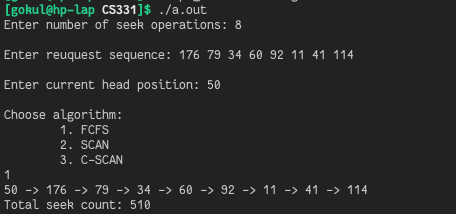
\includegraphics[]{img/p2/ss1.png} \\
    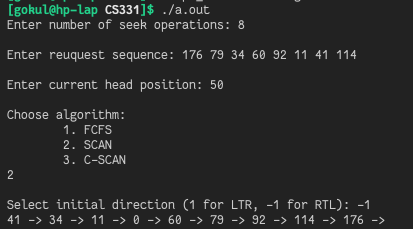
\includegraphics[]{img/p2/ss2.png} \\
    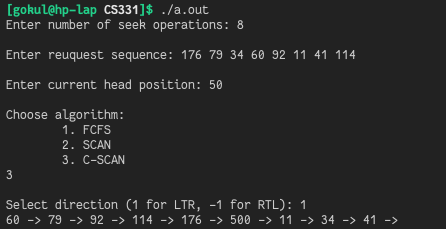
\includegraphics[]{img/p2/ss3.png} 
    
\Large
\section*{Result}
\large
The above algorithms were implemented and its output verified

				\newpage

				\begin{frame}{}
					\centering
					\hspace*{-0.5cm}
					$\vcenter{\hbox{
\includegraphics[width=1.5cm]{img/emblem.jpeg}}}$
					$\vcenter{\resizebox{0.95\textwidth}{!}{
						\begin{tabular}{c}
							 CS333 - System Software Lab $\cdot$ 2020 $\cdot$   \\
							 \hline 
						\end{tabular}
					}}$
				\end{frame}
				\section*{Cycle 1}
\section*{Expt 3}
\begin{center}
    \Large{Page Replacement Algorithms}
\end{center}FCFS
\section*{Aim}
\large
Simulate the following page replacement algorithms.\\
a) FIFO\\
b) LRU \\
c) LFU \\

\section*{Algorithm}
    \subsection*{FIFO}
    \begin{verbatim}
		1 Start traversing the pages .
		2 If set holds less pages than capacity .
		3 Insert page into the set one by one until
		4 the size of set reaches capacity or all
		5 page requests are processed .
		6 Simultaneously maintain the pages in the
		7 queue to perform FIFO .
		8 Increment page fault
		9 Else
		10 If current page is present in set , do nothing .
		11 Else
		12 Remove the first page from the queue
		13 as it was the first to be entered in
		14 the memory
		15 Replace the first page in the queue with
		16 the current page in the string .
		17 Store current page in the queue .
		18 Increment page faults .
		19 Return page faults .
    \end{verbatim}  
    \subsection*{LRU}
    \begin{verbatim}
        1 Start traversing the pages .
		2 If set holds less pages than capacity .
		3 Insert page into the set one by one until
		4 the size of set reaches capacity or all
		5 page requests are processed .
		6 Simultaneously maintain the recent occurred
		7 index of each page in a map called indexes .
		8 Increment page fault
		9 Else
		10 If current page is present in set , do nothing .
		11 Else
		12 Find the page in the set that was least
		13 recently used . We find it using index array .
		14 We basically need to replace the page with
		15 minimum index .
		16 Replace the found page with current page .
		17 Increment page faults .
		18 Update index of current page .
		19 Return page faults .
    \end{verbatim}
    \subsection*{LFU}
    \begin{verbatim}
        1 Start traversing the pages .
		2 If set holds less pages than capacity .
		3 Insert page into the set one by one until
		4 the size of set reaches capacity or all
		5 page requests are processed .
		6 Simultaneously maintain the recent occurred
		7 index of each page in a map called indexes .
		8 Increment page fault
		9 Else
		10 If current page is present in set , do nothing .
		11 Else
		12 Find the page in the set that was least
		13 frequently used . We find it using index array .
		14 We basically need to replace the page with
		15 minimum index .
		16 Replace the found page with current page .
		17 Increment page faults .
		18 Update index of current page .
		19 Return page faults .
    \end{verbatim}  
    
    \section*{Source Code}
    \Large\textbf{fifo}
\small

\begin{lstlisting}[language=C]
void fifo(int * frames, int * pages, size_t n_frames, size_t n_pages)
{
	size_t i, queue = 0;
	int n_faults = 0, n_hits = 0;

	for(i = 0; i < n_pages; i++)
	{
		printf("\nCurrent page: %d", pages[i]);

		if(! contains(frames, n_frames, pages[i]))
		{
			frames[queue] = pages[i];
			++n_faults;
			printf("\nFault");
			queue = (queue+1) % n_frames;
		}
		else
		{
			++n_hits;
			printf("\nHit");
		}
		
		printf("\nFrames: ");
		print_arr(frames, n_frames);
	}

	printf("\nNumber of pages faults: %d\n", n_faults);
}
    \end{lstlisting}
    
        \Large\textbf{lru}
\small

\begin{lstlisting}[language=C]
int find_lru(int * last_used, int n)
{
	int lru = 0, lru_count = 0;

	for(size_t i = 0; i < n; ++i)
	{
		if(last_used[i] < lru_count)
		{
			lru_count = last_used[i];
			lru = i;
		}
		++i;
	}

	return lru;
}

void lru(int * frames, int * pages, size_t n_frames, size_t n_pages)
{
	size_t i, index;
	int n_hits = 0, n_faults = 0;
	int * last_used = malloc(n_frames * sizeof(int));

	for(i = 0; i < n_frames; i++) last_used[i] = 0;

	for(i = 0; i < n_pages; i++)
	{
		printf("\nCurrent page: %d", pages[i]);

		if(!(index = contains(frames, n_frames, pages[i])))
		{
			if(i < n_frames) index = i;
			
			else {
				index = find_lru(last_used, n_frames);
			}

			++n_faults;
			printf("\nFault");
			frames[index] = pages[i];
		}
		else
		{
			++n_hits;
			printf("\nHit");
		}
		last_used[index] = n_faults + n_hits;
		printf("\nFrames: ");
		print_arr(frames, n_frames);
	}

	printf("\nNumber of faults: %d\n", n_faults);
}
    \end{lstlisting}
        \Large\textbf{lfu}
\small

\begin{lstlisting}[language=C]
int find_lfu(int * freq_used, int n)
{
	int lfu = 0, lfu_count = 0;

	for(size_t i = 0; i < n; ++i)
	{
		if(freq_used[i] < lfu_count)
		{
			lfu_count = freq_used[i];
			lfu = i;
		}
		++i;
	}

	return lfu;
}

void lfu(int * frames, int * pages, size_t n_frames, size_t n_pages)
{
	size_t i, index;
	int n_hits = 0, n_faults = 0;
	int * freq_used = malloc(n_frames * sizeof(int));

	for(i = 0; i < n_frames; i++) freq_used[i] = 0;

	for(i = 0; i < n_pages; i++)
	{
		printf("\nCurrent page: %d", pages[i]);

		if(!(index = contains(frames, n_frames, pages[i])))
		{
			if(i < n_frames) index = i;
			
			else {
				index = find_lfu(freq_used, n_frames);
			}

			++n_faults;
			printf("\nFault");
			frames[index] = pages[i];
		}
		else
		{
			++n_hits;
			printf("\nHit");
		}
		freq_used[index]++;
		printf("\nFrames: ");
		print_arr(frames, n_frames);
	}

	printf("\nNumber of faults: %d\n", n_faults);
}
	
    \end{lstlisting}
    \section*{Output}
    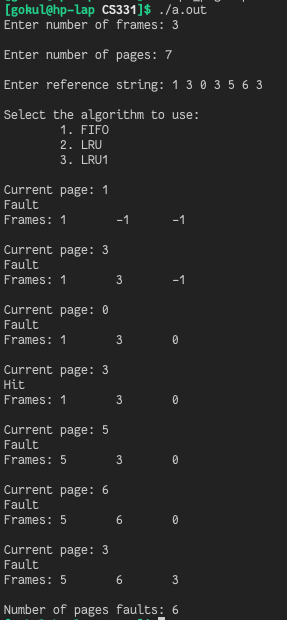
\includegraphics[]{img/p3/ss1.png} \\
    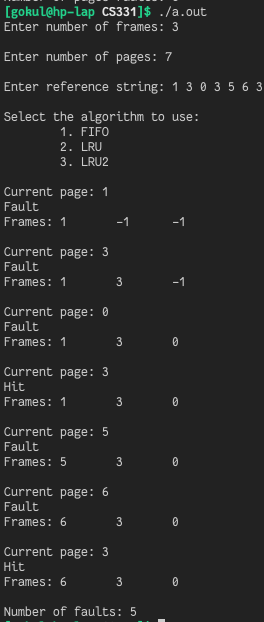
\includegraphics[]{img/p3/ss2.png} \\
    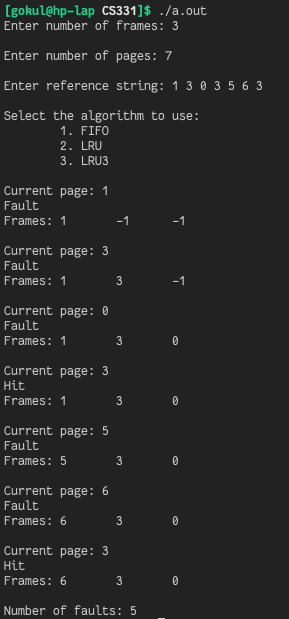
\includegraphics[]{img/p3/ss3.png} 
    
\Large
\section*{Result}
\large
The above algorithms were implemented and its output verified
					\newpage

\begin{frame}{}
	\centering
	\hspace*{-0.5cm}
	$\vcenter{\hbox{
\includegraphics[width=1.5cm]{img/emblem.jpeg}}}$
	$\vcenter{\resizebox{0.95\textwidth}{!}{
		\begin{tabular}{c}
			 CS333 - System Software Lab $\cdot$ 2020 $\cdot$   \\
			 \hline 
		\end{tabular}
	}}$
\end{frame}
\section*{Cycle 1}
\section*{Expt 4}
\begin{center}
	\Large{Banker\'s Algorithm}
\end{center}FCFS
\section*{Aim}
\large
Implement the banker’s algorithm for deadlock avoidance.

\section*{Algorithm}
	\begin{verbatim}
		Implement the banker’s algorithm for deadlock avoidance.
	\end{verbatim}  
	\subsection*{LRU}
	\begin{verbatim}
	1 If Requesti = Needi , go to step 2. Otherwise , raise an error
	condition ,
	2 since the process has exceeded its maximum claim .
	3 If Requesti = Available , go to step 3. Otherwise , Pi must wait ,
	since the
	4 resources are not available .
	5 Have the system pretend to have allocated the requested resources
	to
	6 process , Pi by modify the state as follows :
	7 Available = Available - Requesti ;
	8 Allocationi = Allocationi + Requesti ;
	9 Needi = Needi - Requesti ;
	\end{verbatim}

\section*{Source Code}
\small

\begin{lstlisting}[language=C]
#include <string.h>
#include <stdio.h>
#include <stdlib.h>

#define PROC_NO 5
#define RES_NO 3

struct Process
{
	char *proc_name;
	int *current_alloc;
	int *max_req;
	int finished;
};

int tot_res[3] = {10, 5, 7};

struct Process *create_process()
{
	/* Reads process details */

	struct Process *process = malloc(sizeof(struct Process));
	int *current_alloc = malloc(3 * sizeof(int));
	int *max_req = malloc(3 * sizeof(int));
	process->proc_name = malloc(20 * sizeof(char));

	printf("Enter process name: ");
	scanf("%[^\n]%*c", process->proc_name);

	printf("Enter current allocations of A, B and C: ");
	scanf("%d %d %d%*c", current_alloc, (current_alloc + 1), (current_alloc + 2));

	printf("Enter maximum requirements: ");
	scanf("%d %d %d%*c", max_req, max_req + 1, max_req + 2);

	process->current_alloc = current_alloc;
	process->max_req = max_req;
	process->finished = 0;

	return process;
}

struct Process **get_processes()
{
	/* Returns the process table */

	int i;
	struct Process **proc_table = malloc(PROC_NO * sizeof(struct Process));
	for(i = 0; i < PROC_NO; i++)
		proc_table[i] = create_process();
	
	return proc_table;
}

int *get_requests(struct Process **proc_table)
{
	/* Reads resource request from a process */

	int i, j, req;
	int *req_table = malloc(PROC_NO * RES_NO * sizeof(int));

	for(i = 0; i < PROC_NO; i++)
	{
		printf("Request for %s: ", proc_table[i]->proc_name);
		for(j = 0; j < RES_NO; j++)
		{
			scanf("%d", &req);
			*(req_table + i*RES_NO + j) = req;
		}
			
		printf("\n");
	}

	return req_table;
}



int *calculate_available(struct Process **proc_table) 
{
	/* Calculate the remaining resources */

	int *avialable = malloc(3 * sizeof(int)), i, j, sum;

	for(i = 0; i < RES_NO; i++)
	{
		sum = 0;
		for(j = 0; j < PROC_NO; j++)
			sum += proc_table[j]->current_alloc[i];

		avialable[i] = tot_res[i] - sum;
	}

	return avialable;
} 

int is_safe(struct Process **proc_table, int *available, char *seq)
{
	/* Check if the system is safe and to store the sequence of 
	allocation */

	int i = 0, j, repeat = 0, is_finished = 1, finished_count = 0, need;

	for(i = 0; i < PROC_NO; i++)
	{
		if(!proc_table[i]->finished)
		{
			is_finished = 1;
			for(j = 0; j < RES_NO; j++)
			{
				need = proc_table[i]->max_req[j] - proc_table[i]->current_alloc[j];
				is_finished = is_finished && (available[j] >= need);
			}

			if(is_finished)
			{
				repeat = 1;
				for(j = 0; j < RES_NO; j++)
					available[j] += proc_table[i]->current_alloc[j];
				proc_table[i]->finished = 1;
				strcat(seq, proc_table[i]->proc_name);
				finished_count++;
				strcat(seq, (finished_count != PROC_NO) ? " -> " : "");
			}
		}

		if(i == PROC_NO-1 && repeat)
		{
			i = -1;
			repeat = 0;
		}
	}

	return finished_count == PROC_NO;
}


int main()
{
	struct Process** proc_table = get_processes();
	int i = 0, *avialable;

	char *s = malloc(30 * sizeof(char));
	
	avialable = calculate_available(proc_table);

	if(is_safe(proc_table, avialable, s))
		printf("The system is safe\n%s\n", s);
	else
		printf("The system is unsafe\n");

	free(proc_table);
	free(avialable);
	free(s);
}
	\end{lstlisting}
	\section*{Output}
	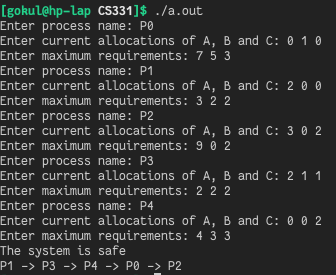
\includegraphics[]{img/p4.png}
	
\Large
\section*{Result}
\large
The banker's algorithm were implemented and its output verified
\newpage
\begin{frame}{}
	\centering
	\hspace*{-0.5cm}
	$\vcenter{\hbox{
\includegraphics[width=1.5cm]{img/emblem.jpeg}}}$
	$\vcenter{\resizebox{0.95\textwidth}{!}{
		\begin{tabular}{c}
			 CS333 - System Software Lab $\cdot$ 2020 $\cdot$   \\
			 \hline 
		\end{tabular}
	}}$
\end{frame}
\section*{Cycle 1}
\section*{Expt 5}
\begin{center}
    \Large{Producer Consumer Problem}
\end{center}
\section*{Aim}
\large
To implement the producer-consumer problem using semaphores

\section*{Algorithm} 
    \subsection*{Producer}
    \begin{verbatim}
		1 do
		2 {
		3 // wait until empty > 0 and then decrement empty
		4 wait ( empty ) ;
		5 // acquire lock
		6 wait ( mutex ) ;
		7 /* perform the insert operation in a slot */
		8 // release lock
		9 signal ( mutex ) ;
		10 // increment full
		11 signal ( full ) ;
		12 }
		13 while ( TRUE )
	\end{verbatim}

	\subsection*{Consumer}
	\begin{verbatim}
		1 do
		2 {
		3 // wait until full >0 and then decrement full
		4 wait ( full ) ;
		5 // acquire the lock
		6 wait ( mutex ) ;
		7 /* perform the remove operation in a slot */
		8 // release the lock
		9 signal ( mutex ) ;
		10 // increment empty
		11 signal ( empty ) ;
		12 }
		13 while ( TRUE )
	\end{verbatim}

\section*{Source Code}
\small

\begin{lstlisting}[language=C]
/* Implement the producer-consumer problem using semaphores */
#include <stdio.h>
#include <stdlib.h>

int mutex = 1;
int full = 0, empty = 3, x = 0;

int wait(int);
int signal(int);
void producer();
void consumer();

int wait(int s)
{
	return --s;
}

int signal(int s)
{
	return ++s;
}

void producer()
{
	mutex = wait(mutex);
	full = signal(full);
	empty = wait(empty);
	++x;
	printf("\nItem%d produced", x);
	mutex = signal(mutex);
}

void consumer()
{
	mutex = wait(mutex);
	full = wait(full);
	empty = signal(empty);
	printf("\nItem%d consumed", x);
	--x;
	mutex = signal(mutex);
}

int main()
{
	int n;
	do {
		printf("\n1. Producer\n2. Consumer\n");
		scanf("%d", &n);
		switch(n)
		{
			case 1:
				if(mutex == 1 && empty) producer();
				else printf("\nBuffer overflow");
				break;

			case 2:
				if(mutex == 1 && full) consumer();
				else printf("\nBuffer empty");
				break;
			
			default:
				printf("\nUnknown command");
				exit(0);
		} 
	} while(1);

	return 0;
}
    \end{lstlisting}
    \section*{Output}
    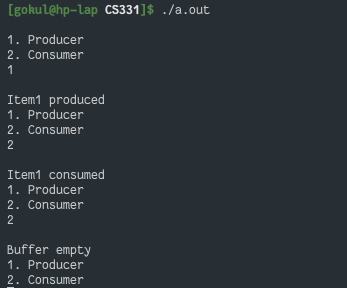
\includegraphics[]{img/p5.png}
    
\Large
\section*{Result}
\large
The producer-consumer problem were solved using semaphores and its output verified
							\newpage

\begin{frame}{}
	\centering
	\hspace*{-0.5cm}
	$\vcenter{\hbox{
\includegraphics[width=1.5cm]{img/emblem.jpeg}}}$
	$\vcenter{\resizebox{0.95\textwidth}{!}{
		\begin{tabular}{c}
			 CS333 - System Software Lab $\cdot$ 2020 $\cdot$   \\
			 \hline 
		\end{tabular}
	}}$
\end{frame}
\section*{Cycle 1}
\section*{Expt 6}
\begin{center}
    \Large{Dining Philosophers Problem}
\end{center}
\section*{Aim}
\large
To implement a program to simulate the working of the dining
philosopher’s problem.

\section*{Algorithm} 
    \begin{verbatim}
		1 process P [ i ]
		2 while true do
		3 { THINK ;
		4 PICKUP ( CHOPSTICK [ i ] , CHOPSTICK [ i +1 mod 5]) ;
		5 EAT ;
		6 PUTDOWN ( CHOPSTICK [ i ] , CHOPSTICK [ i +1 mod 5])
	\end{verbatim}

\section*{Source Code}
\small

\begin{lstlisting}[language=C]

#include <stdio.h>
#include <semaphore.h>
#include <pthread.h>
#include <unistd.h>

#define N 5

typedef enum {
	THINKING,
	HUNGRY,
	EATING
} Actions;

#define LEFT (phil_num + 4) % N
#define RIGHT (phil_num + 1) % N

sem_t mutex;
sem_t S[N];

Actions state[N];
int philosophers[N] = {0, 1, 2, 3, 4}; 

void * philosopher(void *);
void start_eating(int);
void end_eating(int);
void test(int);

void * philosopher(void * num)
{
	while(1)
	{
		int * i = num;
		sleep(1);
		start_eating(*i);
		sleep(0);
		end_eating(*i);
	}
}

void start_eating(int phil_num)
{
	sem_wait(&mutex);
	state[phil_num] = HUNGRY;
	printf("\nPhilosopher%d is hungry", phil_num+1);
	test(phil_num);
	sem_post(&mutex);
	sem_wait(&S[phil_num]);
	sleep(1);
}

void end_eating(int phil_num)
{
	sem_wait(&mutex);
	state[phil_num] = THINKING;
	printf(
		"\nPhilosopher%d stops eating and puts fork %d and %d down",
		phil_num+1,
		LEFT+1,
		phil_num+1
	);
	printf("\nPhilosopher%d is thinking", phil_num+1);
	test(LEFT);
	test(RIGHT);
	sem_post(&mutex);
}

void test(int phil_num)
{
	if(state[phil_num] == HUNGRY && state[LEFT] != EATING && state[RIGHT] != EATING)
	{
		state[phil_num] = EATING;
		sleep(2);
		printf(
			"\nPhilosopher%d takes fork %d and %d",
			phil_num+1,
			LEFT+1,
			phil_num+1
		);
		printf("\nPhilosopher%d is eating", phil_num+1);
		test(LEFT);
		test(RIGHT);
		sem_post(&S[phil_num]);
	}
}

int main()
{
	int i;
	pthread_t thread_id[N];
	sem_init(&mutex, 0, 1);

	for(i = 0; i < N; i++) sem_init(&S[i], 0, 0);

	for(i = 0; i < N; i++)
	{
		pthread_create(&thread_id[i], NULL, philosopher, &philosophers[i]);
		printf("\nPhilosopher%d is thinking", i+1);
	}

	for(i = 0; i < N; i++) pthread_join(thread_id[i], NULL);
}
    \end{lstlisting}
    \section*{Output}
    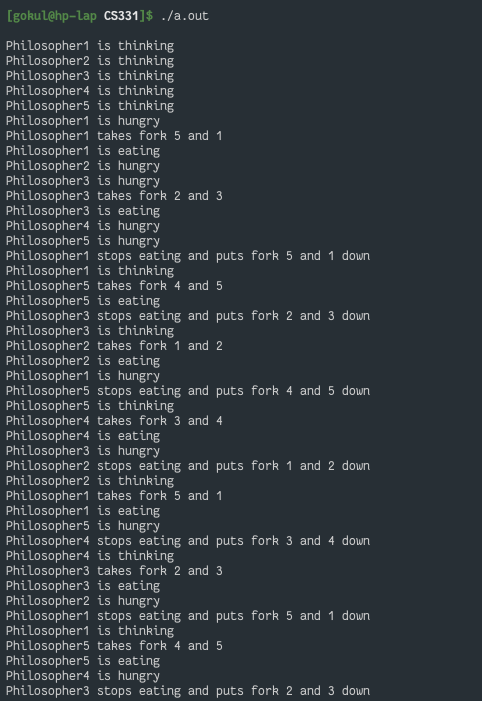
\includegraphics[]{img/p6.png}
    
\Large
\section*{Result}
\large
The dining philosophers problem was solved using semaphores and its output is verified

								\newpage

								\begin{frame}{}
									\centering
									\hspace*{-0.5cm}
									$\vcenter{\hbox{
\includegraphics[width=1.5cm]{img/emblem.jpeg}}}$
									$\vcenter{\resizebox{0.95\textwidth}{!}{
										\begin{tabular}{c}
											 CS333 - System Software Lab $\cdot$ 2020 $\cdot$   \\
											 \hline 
										\end{tabular}
									}}$
								\end{frame}
\section*{Cycle 1}
\section*{Expt 7}
\begin{center}
	\Large{File Organisation Techniques}
\end{center}
\section*{Aim}
\large
Simulate the following file organization techniques:\\
 a) Single level directory\\
 b) Two level directory\\
 c) Hierarchical\\
\section*{Algorithm} 
\subsection{Single Level}
In a single-level directory system, all the files are placed in one directory. There
is a root directory which has all files. It has a simple architecture and there are no
sub directories. Advantage of single-level directory system is that it is easy to find
a file in the directory. A single-level directory has significant limitations, however,
when the number of files increases or when the system has more than one user. Since
all files are in the same directory, they must have unique names.
\subsection{Two Level}
In the two-level directory system, each user has own user file directory (UFD).
The system maintains a master block that has one entry for each user. This master
block contains the addresses of the directory of the users. When a user job starts
or a user logs in, the system’s master file directory (MFD) is searched. When a
user refers to a particular file, only his own UFD is searched. This effectively solves
the name collision problem and isolates users from one another. Isolation is an ad-
vantage when the users are completely independent but is a disadvantage when the
users want to cooperate on some task and to access one another’s files.
\subsection{Hierarchical}
Hierarchical directory structure, also called a tree-structured directory allows
users to create their own subdirectories and to organize their files accordingly. A
tree is the most common directory structure. The tree has a root directory, and
every file in the system has a unique path name. A directory (or subdirectory)
contains a set of files or subdirectories.


\section*{Source Code}
\small
\subsection{FSObject.h}
\begin{lstlisting}[language=C]
#ifndef _FSOBJECT
#define _FSOBJECT

#define MAX_CHILDREN 25
#define PWD_STACK_LENGTH 100

typedef enum { DIR, FIL } FSObjectType;

typedef enum { SINGLE, DOUBLE, HIERARCHIAL } FilesystemType;

struct FileSystemObject {
  char name[255];
  FSObjectType type;
  struct FileSystemObject *children[MAX_CHILDREN];
  int no_of_children;
};

typedef struct FileSystemObject FSObject;

typedef struct {
  FSObject *root;
  FSObject *wd[PWD_STACK_LENGTH];
  int pwd_depth;
  FilesystemType fs_type;
} Filesystem;

void pwd(Filesystem *);
void mkdir(Filesystem *, char[255]);
void cd(Filesystem *, char[255]);
void touch(Filesystem *, char[255]);
void ls(Filesystem *);

#endif
	\end{lstlisting}
\subsection{FSObject.c}
\begin{lstlisting}[language=C]
#include "FSObject.h"
#include <stdio.h>
#include <stdlib.h>
#include <string.h>

// Prints the location of present directory
void pwd(Filesystem *fs) {
  printf("/");
  for (int i = 0; i < (fs->pwd_depth) + 1; i++) {
	printf("%s/", fs->wd[i]->name);
  }
}

// Creates a new directory in pwd
void mkdir(Filesystem *fs, char name[255]) {
  FSObject *pwd = fs->wd[fs->pwd_depth];

  if (pwd->no_of_children == MAX_CHILDREN || fs->fs_type == SINGLE ||
	  (fs->fs_type == DOUBLE && fs->pwd_depth == 1)) {
	printf("Cannot create a new directory\n");
	return;
  } else {
	FSObject *new_dir = malloc(sizeof(FSObject));
	new_dir->type = DIR;
	strcpy(new_dir->name, name);
	new_dir->no_of_children = 0;

	pwd->children[pwd->no_of_children] = new_dir;
	pwd->no_of_children += 1;
  }
}

// Change directory to a child of pwd
void cd(Filesystem *fs, char name[255]) {
  FSObject *pwd = fs->wd[fs->pwd_depth];

  if (strcmp(name, "..") == 0) {
	fs->pwd_depth -= 1;
  } else if (fs->pwd_depth == PWD_STACK_LENGTH) {
	printf("Cannot cd. Maximum stack length reached\n");
	return;
  } else {
	for (int i = 0; i < pwd->no_of_children; i++) {
	  if (strcmp(pwd->children[i]->name, name) == 0 &&
		  pwd->children[i]->type == DIR) {
		fs->pwd_depth += 1;
		fs->wd[fs->pwd_depth] = pwd->children[i];
		return;
	  }
	}
	printf("No directory named %s in %s\n", name, pwd->name);
  }
}

// Create a new file in pwd
void touch(Filesystem *fs, char name[255]) {
  FSObject *pwd = fs->wd[fs->pwd_depth];

  if (pwd->no_of_children == MAX_CHILDREN) {
	printf("Cannot create file. Max children reached\n");
	return;
  }

  FSObject *new_file = malloc(sizeof(FSObject));
  new_file->type = FIL;
  strcpy(new_file->name, name);

  pwd->children[pwd->no_of_children] = new_file;
  pwd->no_of_children += 1;
}

// List all files and folders in pwd
void ls(Filesystem *fs) {
  FSObject *pwd = fs->wd[fs->pwd_depth];

  for (int i = 0; i < pwd->no_of_children; i++)
	if (pwd->children[i]->type == DIR)
	  printf("%s/\t", pwd->children[i]->name);
	else
	  printf("%s\t", pwd->children[i]->name);

  printf("\n");
  return;
}
	\end{lstlisting}
\subsection{main.c}
\begin{lstlisting}[language=C]
#include "FSObject.h"
#include <stdio.h>
#include <stdlib.h>
#include <string.h>

FSObject *init_root_dir(char name[255]) {
  FSObject *root_folder = malloc(sizeof(FSObject));
  strcpy(root_folder->name, name);
  root_folder->type = DIR;
  root_folder->no_of_children = 0;

  return root_folder;
}

Filesystem *init_fs(FilesystemType fs_type, FSObject *root_folder) {
  Filesystem *filesystem = malloc(sizeof(filesystem));
  filesystem->root = root_folder;
  filesystem->fs_type = fs_type;
  filesystem->wd[0] = root_folder;
  filesystem->pwd_depth = 0;

  return filesystem;
}

int main() {
  int choice;
  char command[5], operand[255];
  Filesystem *filesystem;
  FSObject *root_dir;
  FilesystemType fs_type;

  printf("Enter type of filesystem\n1. Single\t 2. Double\t 3. Hierarchial\n");
  scanf("%d", &choice);

  switch (choice) {
  case 1:
	fs_type = SINGLE;
	break;

  case 2:
	fs_type = DOUBLE;
	break;

  case 3:
	fs_type = HIERARCHIAL;
	break;

  default:
	printf("Unknown type\n");
	exit(0);
  }

  printf("Enter root directory name: ");
  scanf("%s", operand);

  root_dir = init_root_dir(operand);
  filesystem = init_fs(fs_type, root_dir);

  printf("\n\nList of available commands:\n"
		 "pwd\tls\tmkdir\ttouch\tcd\texit\n");

  while (strcmp(command, "exit") != 0) {

	pwd(filesystem);
	printf(">> ");
	scanf("%s", command);

	if (strcmp(command, "pwd") == 0) {
	  pwd(filesystem);
	  printf("\n");
	} else if (strcmp(command, "ls") == 0)
	  ls(filesystem);
	else if (strcmp(command, "touch") == 0) {
	  scanf("%s", operand);
	  touch(filesystem, operand);
	} else if (strcmp(command, "mkdir") == 0) {
	  scanf("%s", operand);
	  mkdir(filesystem, operand);
	} else if (strcmp(command, "cd") == 0) {
	  scanf("%s", operand);
	  cd(filesystem, operand);
	}  else if (strcmp(command, "exit") == 0) {
		continue;
	} else {
	  printf("Unknown command %s\n", command);
	}
	  printf("\n");
  }

  return 0;
}
	\end{lstlisting}
	\section*{Output}
	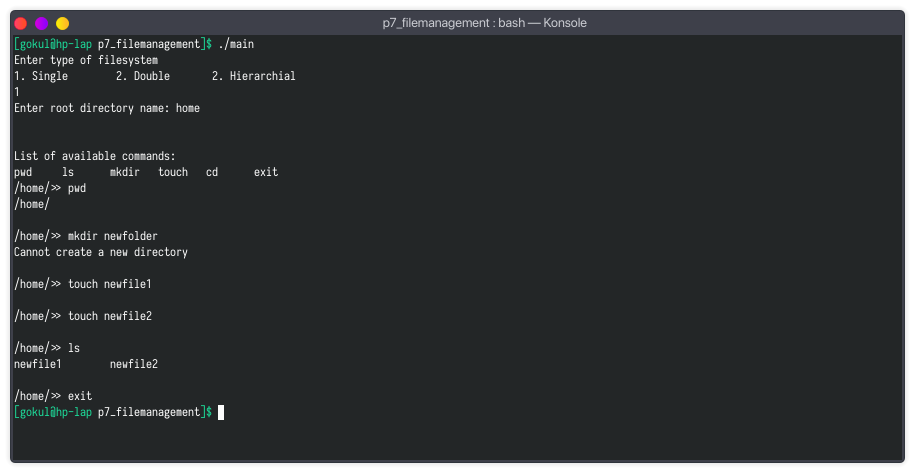
\includegraphics[width=\textwidth]{img/p7/ss1.png}
	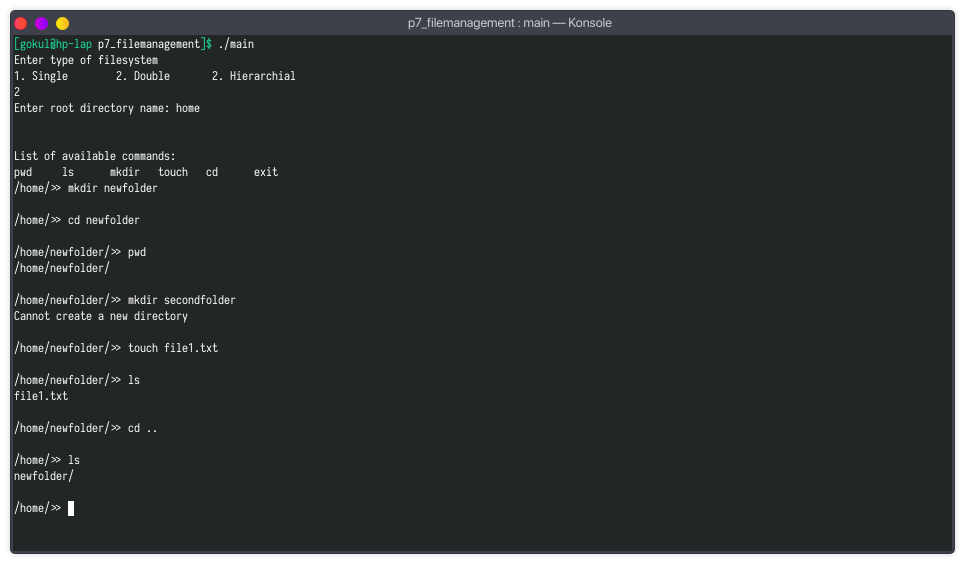
\includegraphics[width=\textwidth]{img/p7/ss2.png}
	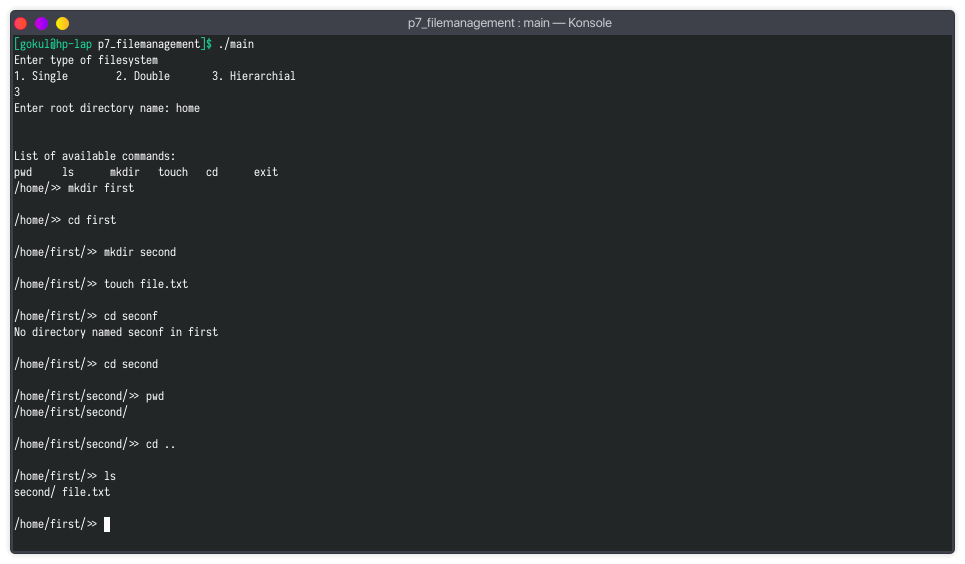
\includegraphics[width=\textwidth]{img/p7/ss3.png}
\Large
\section*{Result}
\large
Basic file organisation techniques was simulated and its output verified
								\newpage

								\begin{frame}{}
									\centering
									\hspace*{-0.5cm}
									$\vcenter{\hbox{
\includegraphics[width=1.5cm]{img/emblem.jpeg}}}$
									$\vcenter{\resizebox{0.95\textwidth}{!}{
										\begin{tabular}{c}
											 CS333 - System Software Lab $\cdot$ 2020 $\cdot$   \\
											 \hline 
										\end{tabular}
									}}$
\end{frame}
\section*{Cycle 2}
\section*{Expt 8}
\begin{center}
	\Large{Pass 1 of a two pass assembler}
\end{center}
\section*{Aim}
\large
Implement pass one of a two pass assembler

\section*{Algorithm} 
	\begin{verbatim}
1 begin
2 read first input line
3 if OPCODE = ’START ’ then
4 begin
5 save #[ OPERAND ] as starting address
6 initialized LOCCTR to starting address
7 write line to intermediate file
8 read next input line
9 end {if START }
10 else
11 initialized LOCCTR to 0
12 while OPCODE != ’END ’ do
13 begin
14 if this is not a comment line then
15 begin
16 if there is a symbol in the LABEL field then
17 begin
18 search SYMTAB for LABEL
19 if found then
20 set error flag ( duplicate symbol )
21 else
22 insert ( LABEL , LOCCTR ) into SYMTAB
23 end {if symbol }
24 search OPTAB for OPCODE
25 if found then
26 add 3 { instruction lengh } to LOCCTR
27 else if OPCODE = ’WORD ’ then
28 add 3 to LOCCTR
29 else if OPCODE = ’RESW ’ then
30 add 3 * #[ OPERAND ] to LOCCTR
31 else if OPCODE = ’RESB ’ then
32 add #[ OPERAND ] to LOCCTR
33 else if OPCODE = ’BYTE ’ then
34 begin
35 find length of constant in bytes
36 add length to LOCCTR
37 end {if BYTE }
38 else
39 set error flag ( invalid operation code )
40 end {if not a comment }
41 write line to intermediate file
42 read next input line
43 end { while not END }
44 write last line to intermediate file
45 save ( LOCCTR - starting address ) as program length
46 end
	\end{verbatim}

\section*{Source Code}
\small

\begin{lstlisting}[language=C]
/* Implement pass one of a two pass assembler */

	\end{lstlisting}
	\begin{verbatim}
input.txt

COPY START 1000
** LDA ALPHA
** ADD ONE
** SUB TWO
** STA BETA
ALPHA BYTE C'KLNCE
ONE RESB 2
TWO WORD 5
BETA RESW 1
** END **
	
optab.txt
LDA 00
STA 23
ADD 01
SUB 05
\end{verbatim}
\section*{Output}
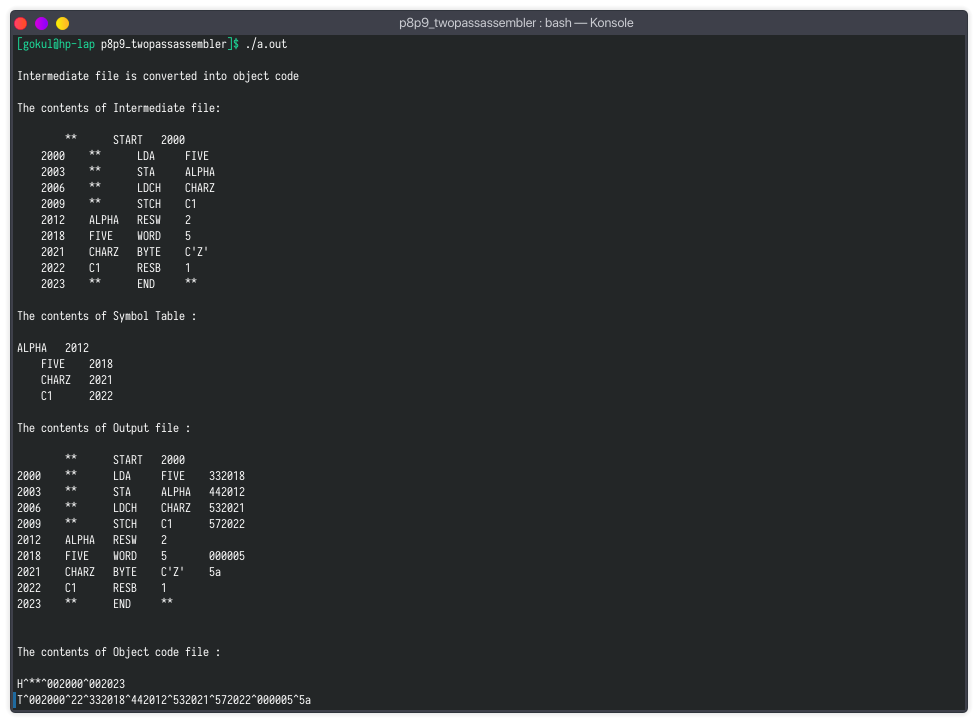
\includegraphics[width=\textwidth]{img/p8.png}
	
\Large
\section*{Result}
\large
The pass one of a two pass assembler was implemented and its output verified

									\newpage

\begin{frame}{}
	\centering
	\hspace*{-0.5cm}
	$\vcenter{\hbox{
\includegraphics[width=1.5cm]{img/emblem.jpeg}}}$
	$\vcenter{\resizebox{0.95\textwidth}{!}{
		\begin{tabular}{c}
			 CS333 - System Software Lab $\cdot$ 2020 $\cdot$   \\
			 \hline 
		\end{tabular}
	}}$
\end{frame}
\section*{Cycle 2}
\section*{Expt 9}
\begin{center}
    \Large{Pass 2 of a two pass assembler}
\end{center}
\section*{Aim}
\large
Implement pass two of a two pass assembler

\section*{Algorithm} 
    \begin{verbatim}
1 begin
2 read first input file { from intermediate file }
3 if OPCODE = ’START ’ then
4 begin
5 write listing line
6 read next input line
7 end {if START }
8 write header record to object program
9 initialized first Text record
10 while OPCODE != ’END ’ do
11 begin
12 if this is not a comment line then
13 begin
14 search OPTAB for OPCODE
15 if found then
16 begin
17 if there is a symbol in OPERAND field then
18 begin
19 search SYMTAB for OPERAND
20 if found then
21 store symbol value as operand address
22 else
23 begin
24 store 0 as operand address
25 set error flag ( undefined symbol )
26 end
27 end {if symbol }
28 else
29 store 0 as operand address
30 assemble the object code instruction
31 end {if opcode found }
32 else if OPCODE = ’BYTE ’ or ’WORD ’ then
33 convert constant to object code
34 if object code not fit into the current Text record then
35 begin
36 write Text record to object program
37 initialized new Text record
38 end
39 add object code to Text record
40 end {if not comment }
41 write listing line
42 read next input line
43 end { while not END }
	\end{verbatim}

\section*{Source Code}
\small

\begin{lstlisting}[language=C]
/* 
  Pass 2 of a Two Pass Assembler
*/

#include <stdio.h>
#include <stdlib.h>
#include <string.h>

void display();

char *my_itoa(int num, char *str)
{
        if(str == NULL)
        {
                return NULL;
        }
        sprintf(str, "%d", num);
        return str;
}

int main()
{
    char a[10], ad[10], label[10], opcode[10], operand[10], symbol[10];
    int start, diff, i, address, add, len, actual_len, finaddr, prevaddr, j = 0;
    char mnemonic[15][15] = {"LDA", "STA", "LDCH", "STCH"};
    char code[15][15] = {"33", "44", "53", "57"};

    FILE *fp1, *fp2, *fp3, *fp4;
    fp1 = fopen("output.txt", "w");
    fp2 = fopen("symtab.txt", "r");
    fp3 = fopen("intermediate.txt", "r");
    fp4 = fopen("objcode.txt", "w");

    fscanf(fp3, "%s\t%s\t%s", label, opcode, operand);

    while (strcmp(opcode, "END") != 0)
    {
        prevaddr = address;
        fscanf(fp3, "%d%s%s%s", &address, label, opcode, operand);
    }
    finaddr = address;
    
    fclose(fp3);
    fp3 = fopen("intermediate.txt", "r");

    fscanf(fp3, "\t%s\t%s\t%s", label, opcode, operand);
    if (strcmp(opcode, "START") == 0)
    {
        fprintf(fp1, "\t%s\t%s\t%s\n", label, opcode, operand);
        fprintf(fp4, "H^%s^00%s^00%d\n", label, operand, finaddr);
        fscanf(fp3, "%d%s%s%s", &address, label, opcode, operand);
        start = address;
        diff = prevaddr - start;
        fprintf(fp4, "T^00%d^%d", address, diff);
    }

    while (strcmp(opcode, "END") != 0)
    {
        if (strcmp(opcode, "BYTE") == 0)
        {
            fprintf(fp1, "%d\t%s\t%s\t%s\t", address, label, opcode, operand);
            len = strlen(operand);
            actual_len = len - 3;
            fprintf(fp4, "^");
            for (i = 2; i < (actual_len + 2); i++)
            {   
                // itoa(operand[i], ad, 16);
                sprintf(ad,"%x",operand[i]);
                fprintf(fp1, "%s", ad);
                fprintf(fp4, "%s", ad);
            }
            fprintf(fp1, "\n");
        }

        else if (strcmp(opcode, "WORD") == 0)
        {
            len = strlen(operand);
            // itoa(atoi(operand), a, 10);
            sprintf(a,"%d",atoi(operand));
            fprintf(fp1, "%d\t%s\t%s\t%s\t00000%s\n", address, label, opcode, operand, a);
            fprintf(fp4, "^00000%s", a);
        }

        else if ((strcmp(opcode, "RESB") == 0) || (strcmp(opcode, "RESW") == 0)) {
            fprintf(fp1, "%d\t%s\t%s\t%s\n", address, label, opcode, operand);
        }

        else
        {
            while (strcmp(opcode, mnemonic[j]) != 0)
                j++;
            if (strcmp(operand, "COPY") == 0)
                fprintf(fp1, "%d\t%s\t%s\t%s\t%s0000\n", address, label, opcode, operand, code[j]);
            else
            {
                rewind(fp2);
                fscanf(fp2, "%s%d", symbol, &add);
                while (strcmp(operand, symbol) != 0)
                    fscanf(fp2, "%s%d", symbol, &add);
                fprintf(fp1, "%d\t%s\t%s\t%s\t%s%d\n", address, label, opcode, operand, code[j], add);
                fprintf(fp4, "^%s%d", code[j], add);
            }
        }

        fscanf(fp3, "%d%s%s%s", &address, label, opcode, operand);
    }

    fprintf(fp1, "%d\t%s\t%s\t%s\n", address, label, opcode, operand);
    fprintf(fp4, "\nE^00%d", start);
    
    fclose(fp4);
    fclose(fp3);
    fclose(fp2);
    fclose(fp1);

    display();
    printf("\n");
    return 0;
}

void display() {
    char ch;
    FILE *fp1, *fp2, *fp3, *fp4;

    printf("\nIntermediate file is converted into object code");

    printf("\n\nThe contents of Intermediate file:\n\n");
    fp3 = fopen("intermediate.txt", "r");
    ch = fgetc(fp3);
    while (ch != EOF)
    {
        printf("%c", ch);
        ch = fgetc(fp3);
    }
    fclose(fp3);

    printf("\n\nThe contents of Symbol Table :\n\n");
    fp2 = fopen("symtab.txt", "r");
    ch = fgetc(fp2);
    while (ch != EOF)
    {
        printf("%c", ch);
        ch = fgetc(fp2);
    }
    fclose(fp2);

    printf("\n\nThe contents of Output file :\n\n");
    fp1 = fopen("output.txt", "r");
    ch = fgetc(fp1);
    while (ch != EOF)
    {
        printf("%c", ch);
        ch = fgetc(fp1);
    }
    fclose(fp1);

    printf("\n\nThe contents of Object code file :\n\n");
    fp4 = fopen("objcode.txt", "r");
    ch = fgetc(fp4);
    while (ch != EOF)
    {
        printf("%c", ch);
        ch = fgetc(fp4);
    }
    fclose(fp4);

}
    \end{lstlisting}
    \begin{verbatim}
input.txt

COPY START 1000
** LDA ALPHA
** ADD ONE
** SUB TWO
** STA BETA
ALPHA BYTE C'KLNCE
ONE RESB 2
TWO WORD 5
BETA RESW 1
** END **
    
optab.txt
LDA 00
STA 23
ADD 01
SUB 05
    \end{verbatim}
    \section*{Output}
    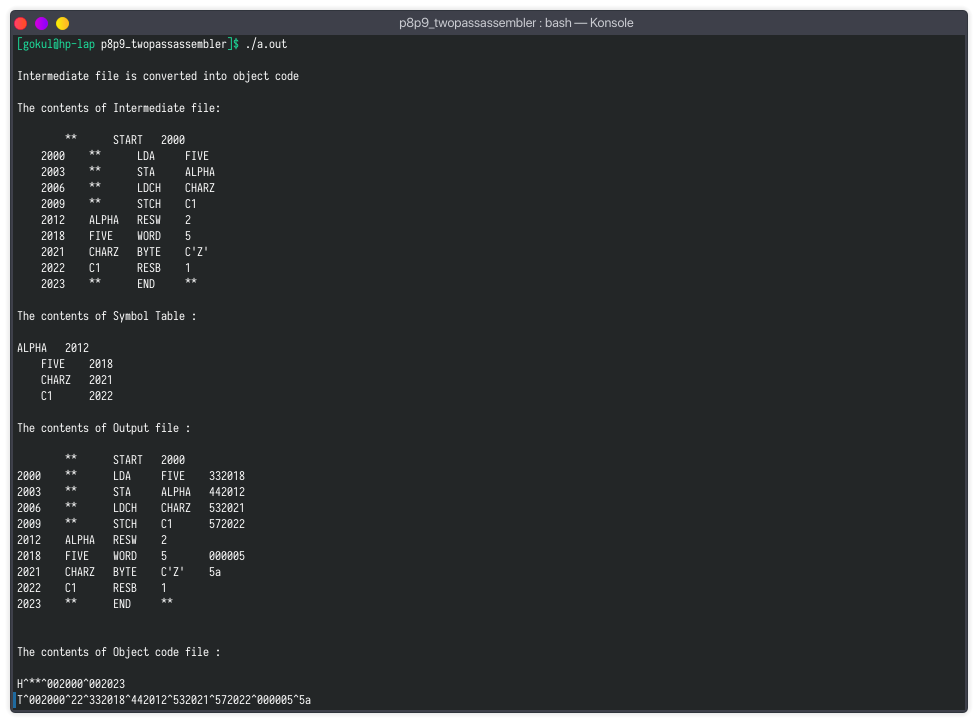
\includegraphics[width=\textwidth]{img/p9.png}
    
\Large
\section*{Result}
\large
The pass two of a two pass assembler was implemented and its output verified

\newpage


\begin{frame}{}
	\centering
	\hspace*{-0.5cm}
	$\vcenter{\hbox{
\includegraphics[width=1.5cm]{img/emblem.jpeg}}}$
	$\vcenter{\resizebox{0.95\textwidth}{!}{
		\begin{tabular}{c}
			 CS333 - System Software Lab $\cdot$ 2020 $\cdot$   \\
			 \hline 
		\end{tabular}
	}}$
\end{frame}
\section*{Cycle 2}
\section*{Expt 10}
\begin{center}
    \Large{One Pass Assembler}
\end{center}
\section*{Aim}
\large
To implement a one pass assembler

\section*{Algorithm} 
    \begin{verbatim}
1 Read first line from the intermediate file .
2 Check to see if the opcode from the first line read is START . If so
then write label , opcode and operand field values of
corresponding statement directly to final output files .
3 Start the following processing for other lines in intermediate file
if it is not a comment line until an END statement is reached .
4 Start writing labels LOCCTR opcode and operand fields of
corresponding statements to the output file along with the
object code .
5 The object code is found by assembling each statement opcode
machine equivalent with the label address .
6 If there is no symbol or label in the operand field , then the
operand address is assigned as zero and it is assembled with
object code of instruction .
7 If OPCODE is BYTE , WORD , RESB etc are convert constants to object
code close operand file and exit .
	\end{verbatim}

\section*{Source Code}
\small

\begin{lstlisting}[language=C]
/* 
	Implement a single pass assembler
*/

#include <stdio.h>
#include <stdlib.h>
#include <string.h>

void itoa(int i, char *a)
{
	sprintf(a, "%d", i);
}

int main()
{
	FILE *input, *optab, *symtab, *symtab2, *output;
	char label[10], opcode[10], operand[10], name[10], optab_code[10], optab_addr[10];
	char symbol[10], symbol_addr[10], locctrs[10], ms[10], q[10], obj1[10], obj2[10];
	int start_address, locctr, prog_len, m[10], i = 0, j = 0, l = 0, k = 0;

	if(! (input = fopen("input.txt", "r")))
	{
		printf("Please make sure input.txt exists\n");
		exit(0);
	}

	if(! (optab = fopen("optab.txt", "r")))
	{
		printf("Please make sure optab.txt exists\n");
		exit(0);
	}

	symtab = fopen("symtab.txt", "w+");
	symtab2 = fopen("symtab2.txt", "w+");
	output = fopen("output.txt", "w+");

	// Checking if input file starts with a START
	fscanf(input, "%s %s %s", label, opcode, operand);
	if(strcmp(opcode, "START") == 0)
	{
		start_address = atoi(operand);
		strcpy(name, label);
		locctr = start_address;
	}

	fscanf(input, "%s %s %s", label, opcode, operand);
	while(strcmp(opcode, "END") != 0)
	{
		if(strcmp(label, "**") == 0)
		{
			while(! feof(optab))
			{
				fscanf(optab, "%s %s", optab_code, optab_addr);
				if(strcmp(optab_code, opcode) == 0)
				{
					m[i++] = locctr + 1;
					fprintf(symtab, "%s **\n", operand);
					fprintf(output, "%s 0000\n", optab_addr);
					locctr += 3;
					break;
				}
			}	
		}
		else
		{
			rewind(symtab);
			while(! feof(symtab))
			{
				fscanf(symtab, "%s %s", symbol, symbol_addr);
				if(strcmp(symbol, label) == 0)
				{
					fprintf(symtab2, "%s %d\n", label, locctr);
					fprintf(output, "%d %d\n", m[j++], locctr);
					++i;
					break;
				}
			}

			if(strcmp(opcode, "RESW") == 0)
				locctr = locctr + 3 * atoi(operand);

			else if(strcmp(opcode, "BYTE") == 0)
			{
				locctr += strlen(operand) - 2;
				for(k = 0; k < strlen(operand); ++k)
					q[l++] = operand[k];

				fprintf(output, "%s **\n", q);
				break; 
			}

			else if(strcmp(opcode, "RESB") == 0)
				locctr += atoi(operand);

			else if(strcmp(opcode, "WORD") == 0)
			{
				locctr += 3;
				fprintf(output, "%s #\n", operand);
				break;
			}
		}

		rewind(optab);
		fscanf(input, "%s %s %s", label, opcode, operand);
	}
	
	fclose(output);
	output = fopen("output.txt", "r");
	prog_len = locctr - start_address;

	printf("H^%s^%d^0%x\n", name, start_address, prog_len);
	printf("T^");
	printf("00%d^0%x", start_address, prog_len);

	while (! feof(output))
	{
		fscanf(output, "%s %s", obj1, obj2);
		if(strcmp(obj2, "0000") == 0)
			printf("^%s%s", obj1, obj2);
		
		else if(strcmp(obj2, "**") == 0)
		{
			printf("^");
			for(k = 0; k < strlen(obj1); k++)
				printf("%d", obj1[k]);
		}

		else if(strcmp(obj2, "#") == 0)
			printf("^%s", obj1);
	}

	rewind(output);
	while (! feof(output))
	{
		fscanf(output, "%s %s", obj1, obj2);
		if(
			strcmp(obj2, "0000") != 0 
			&& strcmp(obj2, "**") != 0 
			&& strcmp(obj2, "#") != 0
		)
			printf("\nT^%s^02^%s", obj1, obj2);
	}
	printf("\nE^00%d\n", start_address);
	return 0;
}
    \end{lstlisting}
    \section*{Output}
    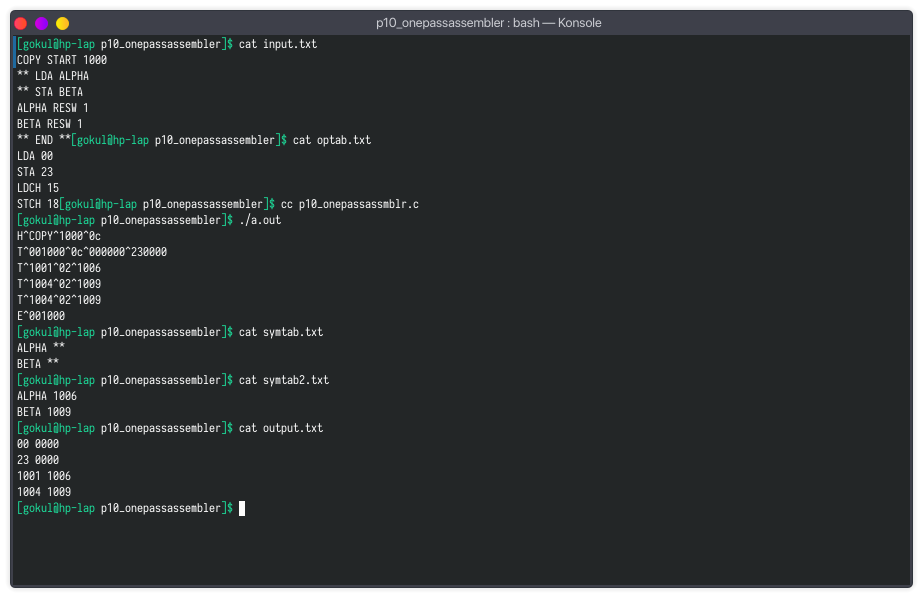
\includegraphics[width=\textwidth]{img/p10.png}
    
\Large
\section*{Result}
\large
One pass assembler is implemented and its output is verified

\newpage


\begin{frame}{}
	\centering
	\hspace*{-0.5cm}
	$\vcenter{\hbox{
\includegraphics[width=1.5cm]{img/emblem.jpeg}}}$
	$\vcenter{\resizebox{0.95\textwidth}{!}{
		\begin{tabular}{c}
			 CS333 - System Software Lab $\cdot$ 2020 $\cdot$   \\
			 \hline 
		\end{tabular}
	}}$
\end{frame}
\section*{Cycle 1}
\section*{Expt 5}
\begin{center}
    \Large{Symbol Table Hashing}
\end{center}
\section*{Aim}
\large
To implement symbol table with hashing

\section*{Algorithm} 
    \begin{verbatim}
1 Start .
2 Define the structure of the Symbol Table
3 Enter the choice for performing the operations in the Symbol Table
4 If the entered choice is 1 , search the symbol table for the symbol
to be
5 inserted . If the symbol is already present , it displays "
Duplicate Symbol ",
6 else , insert the symbol and the corresponding address in the symbol
table .
7 If the entered choice is 2 , delete the particular symbol .
8 If the entered choice is 3 , the symbols present in the symbol table
are
9 displayed .
10 If the entered choice is 4 , the symbol is searched in the symbol
table . If it
11 is not found in the symbol table it displays "Not found ".
12 If the entered choice is 5 , the symbol to be modified is searched
in the
13 symbol table . The address of the label can be modified .
14 Enter choice 6 to exit the program .
15 Stop
	\end{verbatim}

\section*{Source Code}
\small

\begin{lstlisting}[language=C]
	#include <stdio.h>
	#include <stdlib.h>
	#include <string.h>
	
	#define SIZE 20
	
	struct SymTabItem
	{
		char label[10];
		char datatype[10];
		int address;
	
		struct SymTabItem * next;
	};
	
	struct SymTabItem * hash_map[SIZE];
	
	struct SymTabItem * create_item(char label[], char datatype[], int address)
	{
		struct SymTabItem * item;
		item = malloc(sizeof(struct SymTabItem));
		item->address = address;
		strcpy(item->datatype, datatype);
		strcpy(item->label, label);
		item->next = NULL;
	
		return item;
	}
	
	// Hash function presented in K&R version 2
	unsigned calculate_hash(char *s)
	{
		unsigned hashval;
	
		for (hashval = 0; *s != '\0'; s++)
			hashval = *s + 31 * hashval;
	
		return hashval % SIZE;
	}
	
	void insert(char label[], char datatype[], int address)
	{
		unsigned hash = calculate_hash(label);
		struct SymTabItem * curr_item;
		struct SymTabItem * iter = hash_map[hash];
	
		if(iter == NULL)
		{
			hash_map[hash] = create_item(label, datatype, address);
			printf("Insertion successful\n");
			return;
		}
	
		while(iter->next != NULL)
		{
			if(strcmp(iter->label, label) == 0)
			{
				printf("Duplicate symbol\n");
				return;
			}
	
			iter = iter->next;
		}
	
		iter->next = create_item(label, datatype, address);
	}
	
	void delete(char label[])
	{
		unsigned hash = calculate_hash(label);
		struct SymTabItem * prev, * iter;
		prev = iter = hash_map[hash];
	
		while(iter != NULL)
		{
			if(strcmp(iter->label, label) == 0)
			{
				// If the first element is the label
				if(prev == iter) hash_map[hash] = NULL;
				else prev->next = iter->next;
	
				printf("Deleted succesfully\n");
				free(iter);
				return;	
			}
	
			prev = iter;
			iter = iter->next;
		}
	
		printf("No such label present\n");
		return;
	}
	
	void display()
	{
		struct SymTabItem * iter;
	
		for(int i = 0; i < SIZE; i++)
		{
			iter = hash_map[i];
			printf("%d: ", i);
			while(iter != NULL)
			{
				printf(
					"[%s %s %d]",
					iter->label,
					iter->datatype,
					iter->address
				);
	
				iter = iter->next;
			}
			printf("\n");
		}
	}
	
	void search(char label[])
	{
		unsigned hash = calculate_hash(label);
		struct SymTabItem * iter = hash_map[hash];
	
		while(iter != NULL)
		{
			if(strcmp(iter->label, label) == 0)
			{
				printf(
					"Item found\n[%s %s %d]\n",
					iter->label,
					iter->datatype,
					iter->address
				);
				return;
			}
	
			iter = iter->next;
		}
	
		printf("Item not found in symtab\n");
	}
	
	void modify(char label[], int address)
	{
		unsigned hash = calculate_hash(label);
		struct SymTabItem * iter = hash_map[hash];
	
		while(iter != NULL)
		{
			if(strcmp(iter->label, label) == 0)
			{
				iter->address = address;
				printf("Address modified successfully\n");
				return;
			}
	
			iter = iter->next;
		}
	
		printf("Item not found in symtab\n");
	}
	
	int main()
	{
		int choice = 0, address;
		char label[20], datatype[20];
	
		for(int i = 0; i < SIZE; i++) hash_map[i] = NULL;
	
		printf(
			"Enter choice: \n"
			"1. Insertion\n\tformat: 1 label dtype addr\n"
			"2. Deletion\n\tformat: 2 label\n"
			"3. Display\n\tformat: 3\n"
			"4. Search\n\tformat: 4 label\n"
			"5.Modify\n\tformat: 5 label newaddr"
			"6. Quit\n"
		);
		
		do 
		{
			scanf("%d", &choice);
	
			switch (choice)
			{
			case 1:
				scanf(" %s %s %d", label, datatype, &address);
				insert(label, datatype, address);
				break;
			
			case 2:
				scanf(" %s", label);
				delete(label);
				break;
	
			case 3:
				display();
				break;
	
			case 4:
				scanf(" %s", label);
				search(label);
				break;
			
			case 5:
				scanf(" %s %d", label, &address);
				modify(label, address);
				break;
			
			case 6:
				break;
	
			default:
				printf("Unknown choice\n");
			}
		} while(choice != 6);
	}	
    \end{lstlisting}
    \section*{Output}
    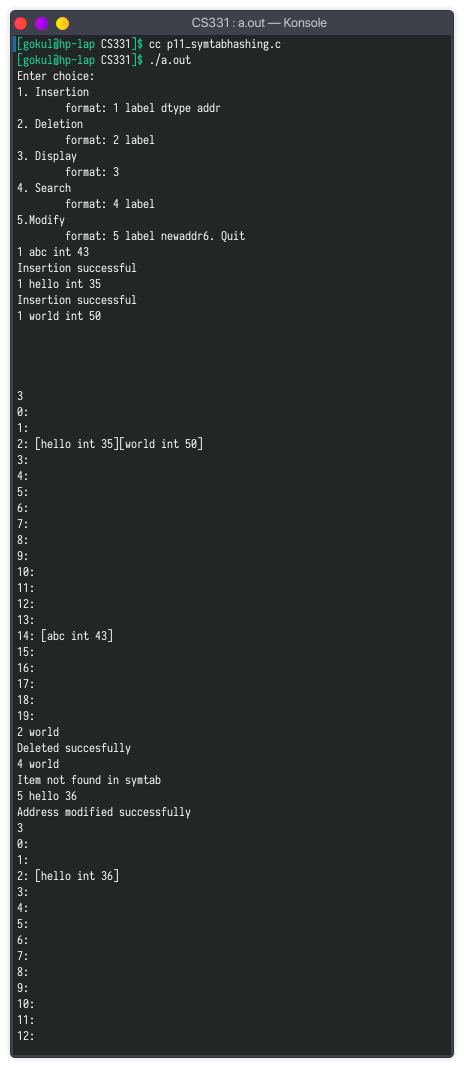
\includegraphics[]{img/p11.png}
    
\Large
\section*{Result}
\large
Symbol table with hashing is implemented and its output is verified
\newpage




\begin{frame}{}
	\centering
	\hspace*{-0.5cm}
	$\vcenter{\hbox{
\includegraphics[width=1.5cm]{img/emblem.jpeg}}}$
	$\vcenter{\resizebox{0.95\textwidth}{!}{
		\begin{tabular}{c}
			 CS333 - System Software Lab $\cdot$ 2020 $\cdot$   \\
			 \hline 
		\end{tabular}
	}}$
\end{frame}
\section*{Cycle 2}
\section*{Expt 5}
\begin{center}
    \Large{Implementation of Absolute Loader}
\end{center}
\section*{Aim}
\large
To implement an absolute loader

\section*{Algorithm} 
    \begin{verbatim}
1 begin
2 read Header record
3 verify program name and length
4 read first Text record
5 while record type != E do
6 begin
7 {if object code is in character form , convert into
8 internal representation }
9 move object code to specified location in memory
10 read next object program record
11 end
12 jump to address specified in End record
13 end
	\end{verbatim}

\section*{Source Code}
\small

\begin{lstlisting}[language=C]
/*  Implement an absolute loader */
#include <stdio.h>
#include <stdlib.h>
#include <string.h>

int main()
{
	FILE * objcode, * output;
	char prgrm_name[20], prgrm_name_in_file[20], * token;
	char code, start_addr[20], total[20], line[50]; 
	int i, start_addri;

	if(! (objcode = fopen("objcode.txt", "r")))
	{
		printf("Please save the object code as objcode.txt");
		exit(0);
	}

	printf("Enter program name: ");
	scanf("%s", prgrm_name);

	// Reading the header record
	fscanf(objcode, "%c^%s", &code, line);
	strcpy(prgrm_name_in_file, strtok(line, "^"));

	// Verifying program name
	if(strcmp(prgrm_name, prgrm_name_in_file) != 0)
	{
		printf("Program name does not match\n");
		exit(0);
	}
	
	while(! feof(objcode))
	{
		fscanf(objcode, "%c^%s", &code, line);
		switch (code)
		{
			case 'T':
				strcpy(start_addr, strtok(line, "^"));
				start_addri = atoi(start_addr);
				
				// Ignoring the length string
				token = strtok(NULL, "^");
				token = strtok(NULL, "^");

				while(token != NULL)
				{
					for(i = 0; i < strlen(token); i += 2)
					{
						printf(
							"%d %c%c\n", 
							start_addri, 
							token[i], 
							token[i+1]
						);
						++start_addri;
					}

					token = strtok(NULL, "^");
				}
				break;
			
			case 'E':
				fclose(objcode);
				return 0;
		}
	}
}	
    \end{lstlisting}
    \section*{Output}
    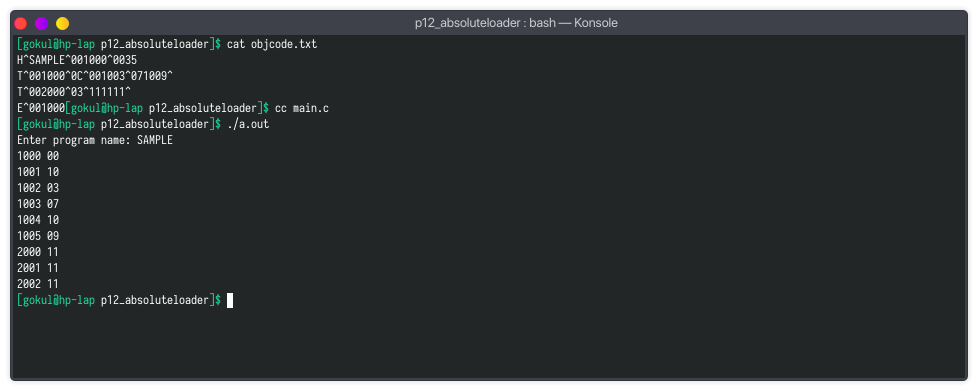
\includegraphics[width=\textwidth]{img/p12.png}
     
\Large
\section*{Result}
\large
Absolute loader is implemented and its output is verified

\newpage


\begin{frame}{}
	\centering
	\hspace*{-0.5cm}
	$\vcenter{\hbox{
\includegraphics[width=1.5cm]{img/emblem.jpeg}}}$
	$\vcenter{\resizebox{0.95\textwidth}{!}{
		\begin{tabular}{c}
			 CS333 - System Software Lab $\cdot$ 2020 $\cdot$   \\
			 \hline 
		\end{tabular}
	}}$
\end{frame}
\section*{Cycle 2}
\section*{Expt 13}
\begin{center}
    \Large{Implementation of Relocating Loader}
\end{center}
\section*{Aim}
\large
To implement a relocating loader

\section*{Algorithm} 
    \begin{verbatim}
1 begin
2 read Header record
3 verify program name and length
4 read first Text record
5 Read the start address of relocation
6 Set addr to start
7 while record type != E do
8 begin
9 read bitmask convert it into binary
10 foreach opcode, address pair if the bit corresponding
  to it in bitmask is 1, relocate the address
11 print addr opcode relocated (or unrelocated) address
12 addr = addr + 3
13 end
14 jump to address specified in End record
15 end
	\end{verbatim}

\section*{Source Code}
\small

\begin{lstlisting}[language=C]
/* Implement a relocating loader */
#include <stdio.h>
#include <stdlib.h>
#include <string.h>

void convert(char[], char[]);

void main()
{
	FILE *objcode;
	int start_addr_in_mem, start_addr_in_prgrm;
	int prgrm_len, line_len, addr = 0, addr_in_mem, i = 0;
	char record_code, prgrm_name[10], prgrm_line[80];
	char *token, bitmask[30], binary_str[120], *opcode;

	if(! (objcode = fopen("objcode.txt", "r")))
	{
		printf("Please save the object code as objcode.txt\n");
		exit(0);
	}

	printf("Enter starting address in memory: ");
	scanf("%x", &start_addr_in_mem);

	while(! feof(objcode))
	{
		fscanf(objcode, "%c", &record_code);
		switch(record_code)
		{
			case 'H':
				fscanf(
					objcode, 
					"^%[^^]^%x^%x", 
					prgrm_name, 
					&start_addr_in_prgrm, 
					&prgrm_len
				);
				break;
			
			case 'T':
				fscanf(
					objcode, 
					"^%x^%x^%[^^]^%s", 
					&addr, 
					&line_len, 
					bitmask, prgrm_line
				);
				addr += start_addr_in_mem;
				convert(bitmask, binary_str);
				
				i = 0;

				// Splitting string with delimiter ^
				token = strtok(prgrm_line, "^");
				while(token != NULL)
				{
					addr_in_mem = (int) strtol(
						strtok(NULL, "^"),
						NULL,
						16
					);

					addr_in_mem = (binary_str[i++] == '0') 
						? addr_in_mem
						: addr_in_mem+start_addr_in_mem;
					printf("%x %s%x\n", addr, token, addr_in_mem);
					addr += 3;
					token = strtok(NULL, "^");
				}
				break;
			
			case 'E':
				exit(0);
		}
	}

	fclose(objcode);
}

void convert(char bitmask[], char binary_str[])
{
	int len = strlen(bitmask);
	strcpy(binary_str, "");
	
	for(int i = 0; i < len; i++)
	{
		switch(bitmask[i])
		{
			case '0':
				strcat(binary_str, "0000");
				break;
			case '1':
				strcat(binary_str, "0001");
				break;
			case '2':
				strcat(binary_str, "0010");
				break;
			case '3':
				strcat(binary_str, "0011");
				break;
			case '4':
				strcat(binary_str, "0100");
				break;
			case '5':
				strcat(binary_str, "0101");
				break;
			case '6':
				strcat(binary_str, "0110");
				break;
			case '7':
				strcat(binary_str, "0111");
				break;
			case '8':
				strcat(binary_str, "1000");
				break;
			case '9':
				strcat(binary_str, "1001");
				break;
			case 'A':
				strcat(binary_str, "1010");
				break;
			case 'B':
				strcat(binary_str, "1011");
				break;
			case 'C':
				strcat(binary_str, "1100");
				break;
			case 'D':
				strcat(binary_str, "1101");
				break;
			case 'E':
				strcat(binary_str, "1110");
				break;
			case 'F':
				strcat(binary_str, "1111");
				break;
		}
	}
} 
	
	\end{lstlisting}
	objcode.txt
	\begin{verbatim}
H^COPY^000000^00107A
T^000000^1E^FFC^14^0033^48^1039^10^0036^28^0030^30^0015^48^1061^3C^0003^20^002A^1C^0039^30^002D
T^002500^15^E00^1D^0036^48^1061^18^0033^4C^1000^80^1000^60^1003
E^000000		
	\end{verbatim}
	
    \section*{Output}
    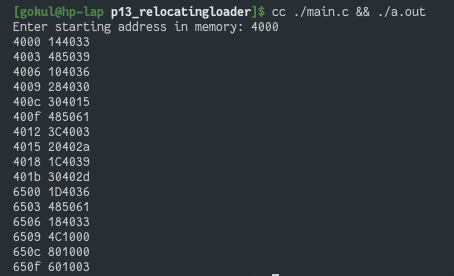
\includegraphics[width=\textwidth]{img/p13.png}
     
\Large
\section*{Result}
\large
Relocating loader is implemented and its output is verified
\newpage


\begin{frame}{}
	\centering
	\hspace*{-0.5cm}
	$\vcenter{\hbox{
\includegraphics[width=1.5cm]{img/emblem.jpeg}}}$
	$\vcenter{\resizebox{0.95\textwidth}{!}{
		\begin{tabular}{c}
			 CS333 - System Software Lab $\cdot$ 2020 $\cdot$   \\
			 \hline 
		\end{tabular}
	}}$
\end{frame}
\section*{Cycle 2}
\section*{Expt 14}
\begin{center}
    \Large{Implementation of Two Pass Macro Processor}
\end{center}
\section*{Aim}
\large
To implement a two pass macro processor

\section*{Algorithm} 
    \begin{verbatim}
Pass-one
1. Scan the input program for MACRO mnemonic
2. If found, add its label to NAMTAB
3. Do until MEND mnemonic is found,
	3.1           child: Text("Feed empty. Pull to refresh"));
	else if (index == 0)
	  return Column(
		mainAxisSize: MainAxisSize.min,
		children: [
		  Text(
			"Pull to refresh",
			style: Theme.of(context)
				.textTheme
				.caption
				.copyWith(fontSize: 10.0),
		  ),
		  buildTitleWidget(),
		],
  Copy the opcode and operand to DEFTAB
	\end{verbatim}

Pass-two
\begin{verbatim}
1. Scan the input program for the macro name mnemonic found in NAMTAB
2. If found, Print the contents of DEFTAB replacing arguments by operands in 1
3. Print the replaced operands to output
4. Else print the label opcode operand to output except for the macro definition
\end{verbatim}

\section*{Source Code}
\small

main.c
\begin{lstlisting}[language=C]
#include <stdio.h>
#include <stdlib.h>
#include <string.h>

void cat(FILE * fp) {
	char line[50];
	rewind(fp);
	while(! feof(fp)) {
		fscanf(fp, "%[^\n]\n", line);
		printf("%s\n", line);
	}
}

void pass_one() {
  FILE *input, *namtab, *deftab;
  char label[20], opcode[20], operand[20];

  if (!(input = fopen("input.txt", "r"))) {
	printf("Please make sure input.txt exists\n");
	exit(0);
  }

  namtab = fopen("namtab.txt", "w+");
  deftab = fopen("deftab.txt", "w+");

  do {
	fscanf(input, "%s %s %s", label, opcode, operand);

	if (strcmp(opcode, "MACRO") == 0) {
	  fprintf(namtab, "%s\n", label);
	  fprintf(deftab, "%s %s\n", label, operand);
	}

	else
	  fprintf(deftab, "%s %s\n", opcode, operand);
	  
  } while (strcmp(opcode, "MEND"));

  printf("Pass one completed\n");
  
  printf("Output of namtab.txt: \n");
  cat(namtab);
  printf("Output of deftab.txt: \n");
  cat(deftab);

  fclose(input);
  fclose(namtab);
  fclose(deftab);
}

void pass_two() {
  FILE *input, *deftab, *namtab, *argtab, *output;
  char label[20], opcode[20], operand[20], macro_name[20], *token;
  char deftab_opcode[20], deftab_operand[20], macro_args[20][20],
	  operand_sub[20];
  size_t macro_args_idx = 0;

  if (!(input = fopen("input.txt", "r")) ||
	  !(deftab = fopen("deftab.txt", "r")) ||
	  !(namtab = fopen("namtab.txt", "r"))) {
	printf("Pass two failed - Verify the output of pass one\n");
  }

  argtab = fopen("argtab.txt", "w+");
  output = fopen("output.txt", "w+");

  fscanf(namtab, "%s", macro_name);

  do {
	fscanf(input, "%s %s %s", label, opcode, operand);

	if (strcmp(opcode, "MACRO") == 0) {
	  token = strtok(operand, ",");
	  while (token != NULL) {
		strcpy(macro_args[macro_args_idx++], token);
		token = strtok(NULL, ",");
	  }

	  while (strcmp(opcode, "MEND") != 0)
		fscanf(input, "%s %s %s", label, opcode, operand);
	}

	token = NULL;

	if (strcmp(opcode, macro_name) == 0) {
	  token = strtok(operand, ",");
	  while (token != NULL) {
		fprintf(argtab, "%s\n", token);
		token = strtok(NULL, ",");
	  }

	  token = NULL;

	  fscanf(deftab, "%s %s", deftab_opcode, deftab_operand);
	  while (strcmp(deftab_opcode, "MEND") != 0) {
		fprintf(output, "- %s ", deftab_opcode);
		token = strtok(deftab_operand, ",");
		while (token != NULL) {
		  if (token[0] == '&') {
			rewind(argtab);
			macro_args_idx = 0;
			while (strcmp(macro_args[macro_args_idx++], token)) {
			  fscanf(argtab, "%s", operand_sub);
			}
			fscanf(argtab, "%s", operand_sub);
			fprintf(output, "%s,", operand_sub);
		  } else {
			  fprintf(output, "%s,", token);
		  }
		  token = strtok(NULL, ",");
		}
		fseek(output, -1, SEEK_CUR); // To remove the trailing comma
		fprintf(output, "\n");
		fscanf(deftab, "%s %s", deftab_opcode, deftab_operand);
	  }
	} else {
		if(strcmp(opcode, "MEND") != 0)
		fprintf(output, "%s %s %s\n", label, opcode, operand);
	}

  } while (strcmp(opcode, "END"));

  printf("\nPass two completed\n");

  printf("Output of argtab.txt");
  cat(argtab);
  printf("Output of output.txt\n");
  cat(output);

  fclose(argtab);
  fclose(deftab);
  fclose(namtab);
  fclose(input);
  fclose(output);
}

void main() {
  pass_one();
  pass_two();
}
\end{lstlisting}
input.txt
\begin{verbatim}
EX1	MACRO &A,&B
-	LDA	&A
-	STA	&B
-	MEND	-
SAMPLE	START	1000
-	EX1	N1,N2
N1	RESW	1
N2	RESW	1
-	END	-	
	\end{verbatim}
	
    \section*{Output}
    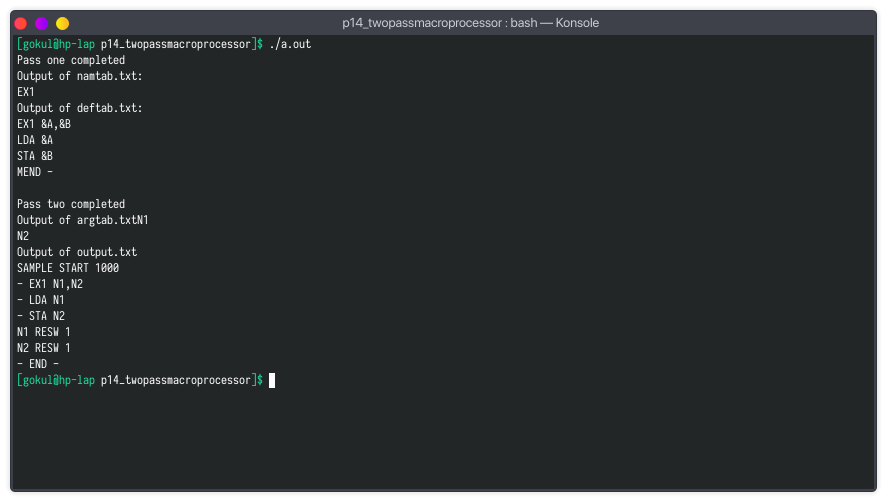
\includegraphics[width=\textwidth]{img/p14.png}
     
\Large
\section*{Result}
\large
Two pass macro processor is implemented and its output is verified
\end{document}